% chapter2.tex - 第二章 局部性质
% 底本: Shafarevich, BAG1, 3rd ed., Book 1 pp.83--146 (PDF pp.99--162).
% 当前包含: §1 奇异点与非奇异点 (PDF pp.99--113).

\chapter{局部性质}

\section{奇异点与非奇异点}

\subsection{点的局部环}

本章研究代数簇中点的局部性质, 即点 $x \in X$ 的在把 $X$ 换成 $x$ 的任何邻域时不变的性质. 既然每点都有仿射邻域, 在研究点的局部性质时可限于仿射簇.

点的最基本局部不变量是它的局部环 $\mathcal O_x$, 由在每个 $x$ 的某邻域中正则的全体函数组成. 不过这个定义需要一点小心, 因为每个函数正则的邻域各不相同.

若 $X$ 不可约, 则 $\mathcal O_x$ 是函数域 $k(X)$ 中由在 $x$ 处正则的全体函数 $f \in k(X)$ 组成的子环. 回忆 $k(X)$ 作为坐标环 $k[X]$ 的分式域的定义, 便知 $\mathcal O_x$ 由形如 $f/g$（$f, g \in k[X]$, $g(x) \ne 0$）的分式组成.

如果我们着眼于这一构造的一般而纯代数的本质, 它会变得更清楚. 它可以应用到任意交换环 $A$ 与 $A$ 的素理想 $\mathfrak p$ 上. 在这个一般性下会出现由 $A$ 中可能的零因子引起的新困难.

考虑满足 $f, g \in A$ 且 $g \notin \mathfrak p$ 的对 $(f, g)$ 所成的集合; 按如下规则把两个对视为相同:
\begin{equation}
	\label{eq:2.1}
	(f, g) = (f', g') \iff \exists\, h \in A \setminus \mathfrak p \text{ 使 } h(fg' - gf') = 0.
\end{equation}
在这个集合上按如下方式定义代数运算:
\begin{equation}
	\label{eq:2.2}
	(f, g) + (f', g') = (fg' + gf',\ gg'), \qquad
	(f, g)(f', g') = (ff',\ gg').
\end{equation}
容易验证这样就得到一个环, 称为 $A$ 在素理想 $\mathfrak p$ 处的局部环, 记作 $A_{\mathfrak p}$.

由 $\varphi(h) = (h, 1)$ 给出的映射 $\varphi: A \to A_{\mathfrak p}$ 是同态. 满足 $g \notin \mathfrak p$ 的元素 $\varphi(g)$ 在 $A_{\mathfrak p}$ 中可逆, 且任一元素 $u \in A_{\mathfrak p}$ 都可写成 $u = \varphi(f)/\varphi(g)$（$g \notin \mathfrak p$）; 我们有时使用略欠精确的记号 $u = f/g$. 形如 $\varphi(f)/\varphi(g)$（$f \in \mathfrak p$, $g \notin \mathfrak p$）的元素组成 $A_{\mathfrak p}$ 的理想 $\mathfrak m$; 而且 $A_{\mathfrak p}$ 中不属于 $\mathfrak m$ 的元素都可逆, 因此 $\mathfrak m$ 包含 $A_{\mathfrak p}$ 的所有其他理想.

于是我们到达了交换代数的基本概念之一: 若环 $\mathcal O$ 有一个理想 $\mathfrak m \subset \mathcal O$, $\mathfrak m \ne \mathcal O$, 且 $\mathfrak m$ 包含 $\mathcal O$ 的所有其他理想, 就称 $\mathcal O$ 为\emph{局部环}.

\begin{lemma}\label{lem:ap-noetherian}
	若 $A$ 是 Noether 环, 则每个局部环 $A_{\mathfrak p}$ 也是.
\end{lemma}

\begin{proof}
	对任意理想 $\mathfrak a \subset A_{\mathfrak p}$, 令 $\bar{\mathfrak a} = \varphi^{-1}(\mathfrak a)$. 这是 $A$ 的理想, 由假设有有限基 $\bar{\mathfrak a} = (f_1, \ldots, f_r)$. 若 $u \in \mathfrak a$, 则 $u = \varphi(f)/\varphi(g)$（$f, g \in A$, $g \notin \mathfrak p$）. 由等同规则 \eqref{eq:2.1}, 存在 $h \in A \setminus \mathfrak p$ 使 $hf \in \bar{\mathfrak a}$; 又因 $1/\varphi(hg) \in A_{\mathfrak p}$, 得 $u \in \varphi(\bar{\mathfrak a}) A_{\mathfrak p} = (\varphi(f_1), \ldots, \varphi(f_r))$. 于是 $\mathfrak a = (\varphi(f_1), \ldots, \varphi(f_r))$, 有有限基. 引理证毕.
\end{proof}

若 $A = k[X]$ 是仿射簇 $X$ 的仿射坐标环而 $\mathfrak p = \mathfrak m_x$ 是点 $x \in X$ 的极大理想, 则 $A_{\mathfrak p}$ 称为 $x$ 的局部环, 记作 $\mathcal O_{X,x}$ 或 $\mathcal O_x$; 由引理它是 Noether 的.

对定义 $\mathcal O_x$ 中元素的每个对 $(f, g)$, 函数 $f/g$ 在 $x$ 的邻域 $D(g)$ 中正则. 规则 \eqref{eq:2.1} 的含义是: 在 $\mathcal O_x$ 中, 我们把在 $x$ 的某邻域（在现在情形即 $D(hgg')$）中相等的函数 $f/g$ 与 $f'/g'$ 等同起来. 于是也可以把 $\mathcal O_x$ 定义为这样的环: 其元素是在 $x$ 的不同邻域中的正则函数, 按刚才所说的规则等同. 这个定义已经不依赖于 $x$ 的某个仿射邻域 $U$ 的选取.

特别地, 我们选取簇 $V$ 使其全部不可约分支都经过 $x$. 那么在 $x$ 的某邻域 $U \subset V$ 上为零的函数 $f$ 在整个 $V$ 上为零. 于是同态 $\varphi: k[V] \to \mathcal O_x$ 是单射, 我们把 $k[V]$ 等同于 $\mathcal O_x$ 的子环. 在这种情形下, 等同规则 \eqref{eq:2.1} 中的因子 $h$ 可以去掉. 换言之, $\mathcal O_x$ 由 $V$ 上的函数组成而不带任何等同, 且所有函数 $\varphi_x \in \mathcal O_x$ 形如 $f/g$（$f, g \in k[V]$, $g(x) \ne 0$）.

类似的构造适用于仿射簇 $X$ 的任何不可约子簇 $Y$: 取 $A = k[X]$ 而 $\mathfrak p = \mathfrak a_Y$. 此时局部环 $A_{\mathfrak p}$ 称为 $X$ 在不可约子簇 $Y$ 处（或沿 $Y$）的局部环, 记作 $\mathcal O_{X,Y}$ 或 $\mathcal O_Y$. 若 $X$ 不可约, 则 $\mathcal O_Y \subset k(X)$ 是由在 $Y$ 的某点正则（从而在 $Y$ 的某个稠密开子集上正则）的全体有理函数组成的环. 极大理想 $\mathfrak m_Y \subset \mathcal O_Y$ 由沿 $Y$ 为零的函数组成, 剩余域 $\mathcal O_Y/\mathfrak m_Y = k(Y)$ 是 $Y$ 的函数域.

过渡到任意拟投影簇 $X$ 的不可约闭子簇 $Y$ 的情形, 与 $Y$ 是一点时同样显然: 此时局部环 $\mathcal O_Y$ 定义为子簇 $Y \cap V$ 的局部环, 其中 $V \subset X$ 是满足 $Y \cap V \ne \emptyset$ 的任意开仿射簇. 局部环不依赖于 $V$ 的选取\footnote{一般地, $\mathcal O_{X,Y}$ 是与 $Y$ 相交的 $X$ 的诸不可约分支 $X_i$ 的函数域 $k(X_i)$ 的直积的子环, 即 $\mathcal O_{X,Y} \subset \prod_{Y \cap X_i \ne \emptyset} k(X_i)$. 也可以把它看成外围空间上在 $Y$ 的稠密开集上正则的有理函数的局部环 $\mathcal O_{\A^N,Y}$ 关于在 $X$ 上为零的函数组成的理想 $\mathfrak a_X \mathcal O_{\A^N,Y}$ 的商. 在讨论第一章那样的有理映射与有理函数时, 要点是: 有理函数定义为分式, 其正则轨迹随后确定; 否则就必须操心定义域不同的两个函数或映射何时相等（例如, 带可去奇点的函数 $z/z$ 等于 $1$ 吗?）.}.

\subsection{切空间}

我们把仿射簇 $X$ 在点 $x$ 处的切空间定义为过 $x$ 且与 $X$ 相切的所有直线组成的集合. 为定义直线 $L \subset \A^N$ 与簇 $X \subset \A^N$ 的相切, 设 $\A^N$ 的坐标系已选好, 使 $x = (0, \ldots, 0) = o$. 于是 $L = \{\, ta \mid t \in k \,\}$, 其中 $a \ne 0$ 是固定点. 为研究 $X$ 与 $L$ 的交, 设 $X$ 由方程组 $F_1 = \cdots = F_m = 0$ 给出, $\mathfrak A_X = (F_1, \ldots, F_m)$.

集合 $X \cap L$ 由方程 $F_1(ta) = \cdots = F_m(ta) = 0$ 给出. 现在处理的是单变量 $t$ 的多项式, 它们的公共根是其最高公因子的根. 设
\begin{equation}
	\label{eq:2.4}
	f(t) = \operatorname{hcf}\bigl(F_1(ta), \ldots, F_m(ta)\bigr) = c \prod (t - \alpha_i)^{k_i}.
\end{equation}
值 $t = \alpha_i$ 对应 $L$ 与 $X$ 的交点. 注意在 \eqref{eq:2.4} 中, 根 $t = \alpha_i$ 带有重数 $k_i$, 它自然解释为 $L$ 与 $X$ 的相交重数. 特别地, 既然 $o \in L \cap X$, \eqref{eq:2.4} 中 $f(t)$ 的根之一是 $t = 0$. 于是得到如下定义.

\begin{definition}[直线与簇的相交重数]\label{def:intersection-mult-line}
	直线 $L$ 与簇 $X$ 在 $o$ 处的\emph{相交重数}, 是 $t = 0$ 作为多项式 $f(t) = \operatorname{hcf}(F_1(ta), \ldots, F_m(ta))$ 的根的重数.
\end{definition}

于是相交重数是整除所有 $F_i(ta)$ 的 $t$ 的最高幂次. 由定义它 $\ge 1$, 因为 $o \in L \cap X$. 若诸 $F_i(ta)$ 恒为零, 则相交重数视为 $+\infty$.

显然 $f(t) = \operatorname{hcf}\{\, F(ta) \mid F \in \mathfrak A_X \,\}$, 故相交重数不依赖于 $\mathfrak A_X$ 的生成元 $F_i$ 的选取.

\begin{definition}[相切]\label{def:tangent-line-def}
	若直线 $L$ 与 $X$ 在 $o$ 处的相交重数 $\ge 2$, 就称 $L$ 在 $o$ 处与 $X$ \emph{相切}.
\end{definition}

现在写出 $L$ 与 $X$ 相切的条件. 既然 $X \ni o$, 每个多项式 $F_i(T)$ 的常数项为 $0$. 对 $i = 1, \ldots, m$, 用 $L_i$ 表示 $F_i$ 的一次项, 于是 $F_i = L_i + G_i$, 其中 $G_i$ 只含次数 $\ge 2$ 的项. 那么 $F_i(at) = t L_i(a) + G_i(ta)$, 而 $G_i(ta)$ 被 $t^2$ 整除. 因此 $F_i(at)$ 被 $t^2$ 整除当且仅当 $L_i(a) = 0$. 于是相切条件为
\begin{equation}
	\label{eq:2.5}
	L_1(a) = \cdots = L_m(a) = 0.
\end{equation}

\begin{definition}[切空间]\label{def:tangent-space}
	在 $x$ 处与 $X$ 相切的直线上的点组成的几何轨迹称为 $X$ 在 $x$ 处的\emph{切空间}\index{qiekongjian@切空间}, 记作 $\Theta_x$; 需要指明簇时记作 $\Theta_{X,x}$.
\end{definition}

于是 \eqref{eq:2.5} 是切空间的方程, 它们表明 $\Theta_x$ 是 $\A^N$ 的线性子空间.

\begin{example}\label{exam:tangent-An}
	$\A^n$ 在任一点的切空间就是 $\A^n$ 自身.
\end{example}

\begin{example}\label{exam:tangent-hypersurface}
	设 $X \subset \A^n$ 是超曲面, $\mathfrak A_X = (F)$. 若 $X \ni o$ 而 $F = L + G$（用上述记号）, 则 $\Theta_o$ 由单个方程 $L(T_1, \ldots, T_n) = 0$ 定义. 于是若 $L \ne 0$ 则 $\dim \Theta_o = n-1$; 若 $L = 0$ 则 $\Theta_o = \A^n$, $\dim \Theta_o = n$. 显然
	\[
		L = \sum \frac{\partial F}{\partial x_i}(0)\, x_i,
	\]
	故对 $n = 2$, 该定义与 \eqref{eq:1.13} 给出的一致.
\end{example}

\begin{example}\label{exam:tangent-node}
	曲线 $y(y - x^2) = 0$ 在 $(0,0)$ 处的切空间是整个 $\A^2$.（尽管它的两个分支有相同的切线 $y = 0$.）
\end{example}

\subsection{切空间的内蕴性}

定义~\ref{def:tangent-space} 是用子簇 $X \subset \A^N$ 的定义方程给出的. 因此, 在同构 $f: X \to Y$ 下, $x$ 与 $f(x)$ 处的切空间同构（即维数相同）这一点并不显然. 我们现在证明它; 为此, 把切空间概念重新表述为只依赖于坐标环 $k[X]$ 的形式.

回忆一些定义. 若 $F(T_1, \ldots, T_N)$ 是多项式而 $x = (x_1, \ldots, x_N)$ 是一点, 则 $F$ 有 Taylor 展开
\[
	F(T) = F(x) + F^{(1)}(T) + \cdots + F^{(k)}(T),
\]
其中诸 $F^{(i)}$ 是变量 $T_j - x_j$ 的 $i$ 次齐次多项式.

线性型 $F^{(1)}$ 称为 $F$ 在 $x$ 处的微分, 记作 $dF$ 或 $d_x F$:
\[
	d_x F = \sum_{i=1}^{N} \frac{\partial F}{\partial T_i}(x)\,(T_i - x_i).
\]
由定义可得
\begin{equation}
	\label{eq:2.6}
	d_x(F + G) = d_x F + d_x G, \qquad d_x(FG) = F(x)\, d_x G + G(x)\, d_x F.
\end{equation}
用这些记号, $X$ 在 $x \in X$ 处的切空间的方程 \eqref{eq:2.5} 可写成
\begin{equation}
	\label{eq:2.7}
	d_x F_1 = \cdots = d_x F_m = 0,
\end{equation}
或
\begin{equation}
	\label{eq:2.8}
	\sum_{i=1}^{N} \frac{\partial F_j}{\partial T_i}(x)\, (T_i - x_i) = 0 \qquad (j = 1, \ldots, m),
\end{equation}
其中 $\mathfrak A_X = (F_1, \ldots, F_m)$. 设 $g \in k[X]$ 定义为多项式 $G$ 在 $X$ 上的限制. 若令 $d_x g = d_x G$, 则答案依赖于多项式 $G$ 的选取; 更确切地说, 它只在不计添加项 $d_x F$（$F \in \mathfrak A_X$）的意义下有定义. 既然 $\mathfrak A_X = (F_1, \ldots, F_m)$, 有 $F = A_1 F_1 + \cdots + A_m F_m$, 由 \eqref{eq:2.6} 与 $F_i(x) = 0$ 得 $d_x F = A_1(x)\, d_x F_1 + \cdots + A_m(x)\, d_x F_m$. 利用 \eqref{eq:2.7} 可见, 对 $F \in \mathfrak A_X$, 所有线性型 $d_x F$ 在 $\Theta_x$ 上为零; 于是, 若把 $d_x g$ 定义为线性型 $d_x G$ 在 $\Theta_x$ 上的限制, 即
\begin{equation}
	\label{eq:2.9}
	d_x g = d_x G \big|_{\Theta_x},
\end{equation}
就得到一个映射, 把每个函数 $g \in k[X]$ 送到 $\Theta_x$ 上一个良定义的线性型 $d_x g$.

\begin{definition}[微分]\label{def:differential}
	由 \eqref{eq:2.9} 定义的线性函数 $d_x g$ 称为 $g$ 在 $x$ 处的\emph{微分}.
\end{definition}

显然,
\begin{equation}
	\label{eq:2.10}
	d_x(f + g) = d_x f + d_x g, \qquad d_x(fg) = f(x)\, d_x g + g(x)\, d_x f.
\end{equation}
于是我们得到同态 $d_x: k[X] \to \Theta_x^*$, 其中 $\Theta_x^*$ 是 $\Theta_x$ 上线性型组成的空间. 既然对 $\alpha \in k$ 有 $d_x \alpha = 0$, 可以用 $d_x: \mathfrak m_x \to \Theta_x^*$ 代替这个映射来研究, 其中 $\mathfrak m_x = \{\, f \in k[X] \mid f(x) = 0 \,\}$ 显然是 $k[X]$ 的理想.

\begin{theorem}\label{thm:differential-iso}
	映射 $d_x$ 给出向量空间 $\mathfrak m_x/\mathfrak m_x^2$ 与 $\Theta_x^*$ 的同构.
\end{theorem}

\begin{proof}
	需要证明 $\operatorname{im} d_x = \Theta_x^*$ 且 $\ker d_x = \mathfrak m_x^2$. 第一点是显然的: $\Theta_x$ 上任何线性型 $\varphi$ 由 $\A^N$ 上某个线性函数 $f$ 诱导, 而 $d_x f = \varphi$.

	为证第二点, 设 $x = (0, \ldots, 0)$ 而 $g \in \mathfrak m_x$ 满足 $d_x g = 0$. 设 $g$ 由多项式 $G \in k[T_1, \ldots, T_N]$ 诱导. 由假设, 线性型 $d_x G$ 在 $\Theta_x$ 上为零, 因此是定义该子空间的方程组 \eqref{eq:2.7} 的线性组合, 即 $d_x G = \lambda_1 d_x F_1 + \cdots + \lambda_m d_x F_m$. 令 $G_1 = G - \lambda_1 F_1 - \cdots - \lambda_m F_m$, 则 $G_1$ 不含 $T_1, \ldots, T_N$ 的 $0$ 次与 $1$ 次项, 故 $G_1 \in (T_1, \ldots, T_N)^2$. 又 $G_1|_X = G|_X = g$, 故 $g \in (t_1, \ldots, t_N)^2$, 其中 $t_i = T_i|_X$. 既然显然 $\mathfrak m_x = (t_1, \ldots, t_N)$, 定理得证.
\end{proof}

众所周知, 若 $L$ 是向量空间而 $M = L^*$ 是 $L$ 上全体线性型组成的空间, 则 $L$ 可以等同于 $M$ 上全体线性型组成的空间, 即 $L = M^*$. 应用于我们的情形, 得到如下结论.

\begin{corollary}\label{cor:cotangent}
	点 $x$ 处的切空间 $\Theta_x$ 同构于 $\mathfrak m_x/\mathfrak m_x^2$ 上全体线性型组成的向量空间.
\end{corollary}

向量空间 $\mathfrak m_x/\mathfrak m_x^2$ 称为 $X$ 在 $x$ 处的\emph{余切空间}.

由此可以对簇之间正则映射 $f: X \to Y$ 下切空间的行为作出推断. 设 $x \in X$ 而 $y = f(x)$. 那么 $f$ 定义映射 $f^*: k[Y] \to k[X]$, 显然 $f^*(\mathfrak m_y) \subset \mathfrak m_x$ 且 $f^*(\mathfrak m_y^2) \subset \mathfrak m_x^2$; 于是 $f$ 诱导映射 $f^*: \mathfrak m_y/\mathfrak m_y^2 \to \mathfrak m_x/\mathfrak m_x^2$. 线性函数与任何函数一样是反变的（沿相反方向映射）, 而由推论~\ref{cor:cotangent}, 切空间 $\Theta_{X,x}$ 与 $\Theta_{Y,y}$ 分别同构于 $\mathfrak m_x/\mathfrak m_x^2$ 与 $\mathfrak m_y/\mathfrak m_y^2$ 上线性型组成的空间, 于是得到映射 $\Theta_{X,x} \to \Theta_{Y,y}$, 称为 $f$ 的\emph{微分}, 记作 $d_x f$.

容易验证, 若 $g: Y \to Z$ 是另一个正则映射而 $z = g(y)$, 则复合映射的微分 $d(g \circ f): \Theta_{X,x} \to \Theta_{Z,z}$ 由 $d(g \circ f) = dg \circ df$ 给出. 若 $f$ 是恒等映射 $X \to X$, 则对每点 $x \in X$, 微分 $d_x f$ 也是切空间上的恒等映射. 这些观察蕴含如下结果.

\begin{corollary}\label{cor:tangent-iso}
	簇的同构把对应点处的切空间变为同构的. 特别地, 一点处切空间的维数在同构下不变.
\end{corollary}

\begin{theorem}\label{thm:tangent-local}
	切空间 $\Theta_{X,x}$ 是簇 $X$ 的点 $x$ 的局部不变量: $\Theta_{X,x}$ 是向量空间 $\mathfrak m_x/\mathfrak m_x^2$ 的对偶空间, 其中 $\mathfrak m_x$ 是 $x$ 的局部环 $\mathcal O_x$ 的极大理想.
\end{theorem}

\begin{proof}
	我们说明如何用 $x$ 的局部环 $\mathcal O_x$ 确定 $\Theta_x$. 回忆有理函数 $F/G$（$F, G \in k[T_1, \ldots, T_n]$, $G(x) \ne 0$）在一点处的微分由
	\[
		d_x(F/G) = \frac{G(x)\, d_x F - F(x)\, d_x G}{G^2(x)}
	\]
	给出. 把函数 $f \in \mathcal O_x$ 视为有理函数 $F/G$ 在 $X$ 上的限制, 定义微分 $d_x f = d_x(F/G)\big|_{\Theta_x}$. 前面在定理~\ref{thm:differential-iso} 之前所作的论证及其证明全部照搬, 便见 $d_x$ 定义了同构 $d_x: \mathfrak m_x/\mathfrak m_x^2 \overset{\sim}{\longrightarrow} \Theta_x^*$, 其中现在 $\mathfrak m_x$ 是局部环 $\mathcal O_x$ 的极大理想 $\{\, f \in \mathcal O_x \mid f(x) = 0 \,\}$. 这就证明了定理~\ref{thm:tangent-local}.
\end{proof}

我们把任意拟投影簇 $X$ 的点 $x$ 处的切空间定义为 $(\mathfrak m_x/\mathfrak m_x^2)^*$, 其中 $\mathfrak m_x$ 是 $x$ 的局部环 $\mathcal O_x$ 的极大理想. 由定理~\ref{thm:tangent-local}, $\Theta_x$ 也是 $x$ 的任何仿射邻域在 $x$ 处的切空间.

这样, 切空间定义为抽象向量空间, 而不实现为任何外围空间的子空间. 不过, 若 $X$ 仿射且 $X \subset \A^N$, 则嵌入 $i: X \hookrightarrow \A^N$ 定义嵌入 $d i: \Theta_{X,x} \hookrightarrow \Theta_{\A^N,x}$. 既然 $\Theta_{\A^N,x}$ 可与 $\A^N$ 等同, 就可以把 $\Theta_{X,x}$ 视为 $\A^N$ 的子空间, 回到 §1.2 给出的定义.

若 $X \subset \PP^N$ 是射影簇而 $x \in X$ 落在仿射块 $\A^N_i$ 中, 则 $\Theta_{X,x}$ 是 $\A^N_i$ 的仿射线性子空间. $\Theta_{X,x}$ 在 $\PP^N$ 中的闭包不依赖于仿射块 $\A^N_i$ 的选取. 尽管对两个不同对象使用同一术语有所含混, 闭包 $\overline{\Theta}_{X,x} \subset \PP^N$ 有时也称为 $X$ 在 $x$ 处的（射影）切空间. 通常的验证表明, $\overline{\Theta}_{X,x} \subset \PP^N$ 由方程
\[
	\sum_{i=0}^{N} \frac{\partial F_\alpha}{\partial \xi_i}(x)\, \xi_i = 0
\]
定义, 其中 $\{F_\alpha\}$ 是 $X$ 的理想的一组齐次基.

切空间的内蕴性为簇嵌入仿射空间的某些问题提供了答案. 例如, 若 $x \in X$ 满足 $\dim \Theta_x = N$, 则 $X$ 不同构于任何 $n < N$ 维仿射空间 $\A^n$ 的子簇: 同构 $f: X \overset{\sim}{\to} Y \subset \A^n$ 将把 $\Theta_x$ 同构地映到子空间 $\Theta_{f(x)} \subset \A^n$. 由此, 对任何 $n > 1$, 可以构造一条曲线 $X \subset \A^n$, 它不同构于任何曲线 $Y \subset \A^m$（$m < n$）. 即取 $X$ 为 $\A^1$ 在映射
\begin{equation}
	\label{eq:2.11}
	x_1 = t^n, \quad x_2 = t^{n+1}, \quad \ldots, \quad x_n = t^{2n-1}
\end{equation}
下的像. 只需证明 $X$ 在 $x = (0, \ldots, 0)$ 处的切空间是整个 $\A^n$, 即所有多项式 $F \in \mathfrak A_X$ 都不含 $T_1, \ldots, T_n$ 的一次项. 设 $F \in \mathfrak A_X$, 写
\[
	F = \sum_{i=1}^{n} a_i T_i + G, \qquad G \in (T_1, \ldots, T_n)^2.
\]
把 \eqref{eq:2.11} 代入 $F$, 得关于 $t$ 的恒等式
\[
	\sum_{i=1}^{n} a_i\, t^{n+i-1} + G(t^n, t^{n+1}, \ldots, t^{2n-1}) \equiv 0.
\]
但若有某个 $a_i \ne 0$, 这是不可能的. 事实上, 项 $a_i t^{n+i-1}$ 的次数 $\le 2n-1$, 而来自 $G(t^n, \ldots, t^{2n-1})$ 的项次数 $\ge 2n$, 二者无法相消.

由刚给出的证明还可知, 曲线 $X$ 在 $x$ 处的任何邻域都不同构于 $\A^m$（$m < n$）中的拟投影簇.

现在给出切空间的一些例子. 先给射影空间 $\PP(V)$（对应于向量空间 $V$）的点处切空间的一个解释. $V$ 在 $v$ 处的切空间 $\Theta_{V,v}$ 可自然地等同于 $V$, 因为 $\mathfrak m_v/\mathfrak m_v^2$ 与 $V$ 上线性型组成的空间（即 $V^*$）的对偶等同. 映射 $\pi: V \setminus 0 \to \PP(V)$, $\pi(\xi_0, \ldots, \xi_n) = (\xi_0 : \cdots : \xi_n)$ 的微分为 $d_v \pi: \Theta_{V,v} = V \to \Theta_{\PP(V),\pi(v)}$. 若在 $v$ 处 $\xi_0 \ne 0$, 则在坐标 $x_i = \xi_i/\xi_0$ 下, 线性型 $\varphi \in \Theta_{V,v}^*$ 变为 $\mathfrak m_{\pi(v)}/\mathfrak m_{\pi(v)}^2$ 上的函数 $\psi = (d_v \pi)(\varphi)$, 满足
\[
	\psi(x_i) = \varphi\, d_v(\xi_i/\xi_0) = \frac{\xi_i\, \varphi(\xi_0) - \xi_0\, \varphi(\xi_i)}{\xi_0^2}.
\]
由此可得, $d_v\pi$ 的像是整个 $\Theta_{\PP(V),\pi(v)}$, 而核由满足 $\xi_i \eta_0 = \xi_0 \eta_i$ 的向量 $(\eta_0, \ldots, \eta_n)$ 组成, 即与 $(\xi_0, \ldots, \xi_n)$ 成比例的向量. 于是对 $\xi \in \PP(V)$ 有
\begin{equation}
	\label{eq:2.12}
	\Theta_{\PP(V),\xi} \cong V / l_\xi,
\end{equation}
其中 $l_\xi = \pi^{-1}(\xi)$ 是点 $\xi \in \PP(V)$ 对应的 $V$ 中直线.

由此可以说, 若 $X \subset \PP(V)$ 是由齐次方程组定义的射影簇, $\widetilde X \subset V$ 是由同样方程定义的 $X$ 上的仿射锥, 则 $\overline\Theta_{X,x} \cong \Theta_{\widetilde X,\widetilde x} / l_x$, 其中 $x = \pi(\widetilde x)$, $l_x$ 如 \eqref{eq:2.12}. 我们把切空间的这一解释应用于例~\ref{exam:grassmannian}--\ref{exam:determinantal} 考虑过的代数簇.

\begin{example}[Grassmann 簇]\label{exam:tangent-grassmann}
	这里只考虑 $X = \operatorname{Grass}(2, n)$. 它由 $\PP(\bigwedge^2 V)$ 中的方程 $x^2 = x \wedge x = 0$ 定义. 对这些方程微分, 得仿射锥 $\widetilde X \subset \bigwedge^2 V$ 在 $x$ 处的切空间由满足
	\begin{equation}
		\label{eq:2.13}
		x \wedge y = 0
	\end{equation}
	的 $y \in \bigwedge^2 V$ 组成. 设 $x \in \bigwedge^2 L \subset \bigwedge^2 V$ 是对应于 $2$ 平面 $L \subset V$ 的点, 即 $\bigwedge^2 L = k x$; 取 $f \in \operatorname{Hom}(L, V/L)$. 那么容易验证, 对 $L$ 的任何基 $e_1, e_2$, 双向量 $y = e_1 \wedge f(e_2) - e_2 \wedge f(e_1)$ 在 $\bigwedge^2 V / kx$ 中唯一确定, 在相差一个标量倍数的意义下不依赖于 $L$ 的基的选取, 且满足 \eqref{eq:2.13}; 反之, \eqref{eq:2.13} 的任何解都这样得到. 于是对任何 $2$ 平面 $L \subset V$,
	\begin{equation}
		\label{eq:2.14}
		\Theta_{\operatorname{Grass}(2,V),L} \cong \operatorname{Hom}(L, V/L).
	\end{equation}
	我们将在原书第 6 章第 4.1 节例 6.24 中证明, 类似的关系对任何 $\operatorname{Grass}(r, V)$ 成立, 并给出其解释.

	我们从 $\operatorname{Grass}(2, V)$ 由方程组 $x \wedge x = 0$ 给出这一事实出发导出 \eqref{eq:2.14}. 但为应用 §1.2 的切空间定义, 需要知道这些方程不只是在集合论意义上定义 $X = \operatorname{Grass}(2, V)$, 而且生成理想 $\mathfrak A_X$. 目前我们只能断言: 若把方程 $x \wedge x = 0$ 写成 $F_1 = \cdots = F_m = 0$, 则在限制到 $\PP(\bigwedge^2 V)$ 的某个仿射块后, 由 $\sum (\partial F_i/\partial T_j)(x)(T_j - x_j) = 0$ 定义的空间同构于 $\operatorname{Hom}(L, V/L)$. 由此已经不难推出 $\mathfrak A_X = (F_1, \ldots, F_m)$, 从而关系 \eqref{eq:2.14} 无保留地成立（见原书第 4 章第 3.3 节习题 15）.
\end{example}

\begin{example}[结合代数的簇]\label{exam:tangent-algebras}
	对结合关系 \eqref{eq:1.28} 微分, 可见结合代数簇的切空间由方程
	\begin{equation}
		\label{eq:2.15}
		\sum_l \bigl( \alpha_{ij}^l\, x_{lk}^m + \alpha_{lk}^m\, x_{ij}^l \bigr) = \sum_l \bigl( \alpha_{il}^m\, x_{jk}^l + \alpha_{jk}^l\, x_{il}^m \bigr)
	\end{equation}
	定义. 设 $x_{ij}^m = \eta_{ij}^m$ 满足这些方程. 考虑由 $f(e_i, e_j) = \sum_m \eta_{ij}^m e_m$ 给出的双线性函数 $f(x, y)$（$x, y \in A$）. 此时关系 \eqref{eq:2.15} 取形式
	\[
		x\, f(y, z) + f(x, yz) = f(xy, z) + f(x, y)\, z \qquad \text{对一切 } x, y, z \in A.
	\]
	这种类型的函数称为 $A$ 上的 $2$-上闭链. 于是, 结合代数簇在对应于代数 $A$ 的点处的切空间同构于 $A$ 上 $2$-上闭链组成的空间.

	与例~\ref{exam:tangent-grassmann} 一样, 我们从只在集合论意义上定义结合代数簇的关系 \eqref{eq:1.28} 出发. 这些方程的左端是否生成该簇的理想, 似乎尚不清楚; 已知对 Lie 代数这不成立, 对结合代数很可能也不成立. 于是, 只有在使 \eqref{eq:1.28} 生成代数簇理想的那些维数 $n$ 下, 或对使这些方程局部生成理想的那些 $A$, $A$ 上 $2$-上闭链的空间才等于代数簇在 $A$ 处的切空间. 不过, 结合关系 \eqref{eq:1.28} 非常自然, 从它们推出的任何信息都应具有某种意义. 特别地, 关于 $2$-上闭链空间的讨论, 见原书第 5 章第 3.4 节与第 6 章第 4.1 节例 6.25.
\end{example}

\begin{example}[二次曲面的簇]\label{exam:tangent-quadrics}
	设 $V$ 是对称 $n \times n$ 矩阵 $A = (x_{ij})$（$x_{ij} = x_{ji}$）组成的向量空间, 考虑由 $\det A = 0$（$A \in V$）定义的簇 $\Delta \subset \PP(V)$. 容易看出 $\det A$ 是不可约多项式, 故 $\Delta$ 是不可约超曲面.

 仿射锥 $\widetilde\Delta$ 在矩阵 $A$ 处的切空间由满足 $\bigl( \frac{d}{dt} \det(A + tB) \bigr)\big|_{t=0} = 0$ 的矩阵 $B \in V$ 组成. 既然
	\[
		\frac{d}{dt} \det(A + tB)\Big|_{t=0} = \det A_1 + \cdots + \det A_n,
	\]
	其中 $A_i$ 是把 $A$ 的第 $i$ 行换成 $B$ 的第 $i$ 行所得的矩阵, 故当 $\operatorname{rank} A < n-1$ 时该表达式为 $0$; 在这些点处 $\Theta_{\Delta,A} = \PP(V)$. 设 $A$ 的秩为 $n-1$. 变换 $A \mapsto {}^t C A C$（$C$ 为非退化矩阵）显然定义 $\Delta$ 的自同构. 用这样的变换可把 $A$ 对应的二次型 $f$ 化为 $x_1^2 + \cdots + x_{n-1}^2$. 于是可设 $f = x_1^2 + \cdots + x_{n-1}^2$, 此时同样的论证表明 $\bigl( \frac{d}{dt}\det(A + tB) \bigr)\big|_{t=0}$ 等于 $B$ 的元素 $b_{nn}$. 故在这样的点处, 切空间 $\Theta_{\Delta,A}$ 可与满足 $b_{nn} = 0$ 的矩阵 $B \in V$ 组成的子空间等同, 即经过奇异二次型 $f = 0$ 的顶点的二次曲面组成的空间.
\end{example}

\subsection{奇异点}

现在来说明, 对不可约拟投影簇 $X$ 的切空间维数可以说些什么. 我们的结果是局部的, 故限于仿射簇.

设 $X \subset \A^N$ 是不可约簇. 考虑直积 $\A^N \times X$ 中由满足 $a \in \Theta_x$ 的对 $(a, x)$（$a \in \A^N$, $x \in X$）组成的子集 $\Theta$. 方程 \eqref{eq:2.7} 表明 $\Theta$ 在 $\A^N \times X$ 中闭. 用 $\pi: \Theta \to X$ 表示第二投影 $\pi(a, x) = x$. 显然 $\pi(\Theta) = X$ 而 $\pi^{-1}(x) = \{\, (a, x) \mid a \in \Theta_x \,\}$. 于是 $\Theta$ 以 $X$ 各点的切空间 $\Theta_x$ 为纤维构成 $X$ 上的纤维化; $\Theta \to X$ 称为 $X$ 的切丛空间. 对 $\Theta$ 应用映射纤维维数的结果（定理~\ref{thm:fibre-dim} 及其推论~\ref{cor:fibre-closed}）, 便知存在数 $s$ 使对一切 $x \in X$ 有 $\dim \Theta_x \ge s$, 而使 $\dim \Theta_y > s$ 的点 $y \in X$ 组成一个真闭子簇 $Y \subsetneq X$, 即维数较小的簇.

\begin{definition}[非奇异点]\label{def:nonsingular-point}
	设 $X$ 是不可约簇, 令 $s = \min_{x \in X} \dim \Theta_x$. 若 $\dim \Theta_x = s$, 就称点 $x \in X$ 为\emph{非奇异}的, 也称 $X$ 在 $x$ 处非奇异; 若 $X$ 在每点 $x \in X$ 都非奇异, 就称簇 $X$ 非奇异. 若 $\dim \Theta_x > s$, 则称 $x$ 为 $X$ 的奇异点\footnote{现代文献中 smooth 与 nonsingular 通用. 本书英文第一版用过的术语 simple 已过时, 它出自 Zariski, 是俄文原文的直译, 现已不用.}.
\end{definition}

如上所见, $X$ 的非奇异点组成非空开子簇, 奇异点组成真闭子簇.

考虑超曲面的例子（例~\ref{exam:tangent-hypersurface}）, 它在 $n = 2$ 的特殊情形包含第一章 §1.5 考虑过的代数平面曲线. 若 $\mathfrak A_X = (F)$, 则切空间在 $x$ 处的方程为
\[
	\sum_{i=1}^{n} \frac{\partial F}{\partial T_i}(x)\, (T_i - x_i) = 0.
\]
我们现在证明此情形 $s = \min \dim \Theta_x = n-1$. 这显然等价于诸 $\partial F/\partial T_i$ 不全在 $X$ 上恒为零. 特征 $0$ 时这将意味着 $F$ 是常数, 特征 $p > 0$ 时意味着各未定元在 $F$ 中只以 $p$ 的倍数次幂出现; 但此时如第一章 §1.5 那样, 既然域 $k$ 代数闭, 将得 $F = F_1^p$, 与 $\mathfrak A_X = (F)$ 矛盾.

于是在我们的例子中, 非奇异点 $x \in X$ 满足 $\dim \Theta_x = \dim X = n-1$. 现在证明对任意不可约簇同样的结论成立, 且一般情形可归结为超曲面的情形.

\begin{theorem}\label{thm:nonsingular-dim}
	非奇异点处切空间的维数等于簇的维数.
\end{theorem}

\begin{proof}
	按非奇异点的定义, 定理断言: 对不可约簇 $X$ 的每点 $x$ 有 $\dim \Theta_x \ge \dim X$, 且使 $\dim \Theta_x = \dim X$ 的点 $x$ 组成非空开集. 这显然是局部断言, 只需考虑仿射簇的情形. 我们已见存在 $s$ 使对一切 $x \in X$ 有 $\dim \Theta_x \ge s$, 且使 $\dim \Theta_x = s$ 的点组成非空开集; 只剩证明 $s = \dim X$. 现在用定理~\ref{thm:birational-hypersurface}: $X$ 双有理等价于某超曲面 $Y$.

	设 $\varphi: X \to Y$ 是定理~\ref{thm:birational-hypersurface} 的双有理映射. 由第一章的命题~\ref{prop:birational-opens}, 存在非空开集 $U \subset X$ 与 $V \subset Y$, 使 $\varphi$ 给出同构 $\varphi: U \overset{\sim}{\to} V$. 由定理陈述前的注记, 簇 $Y$ 的非奇异点集 $W$ 是开集, 且对一切 $y \in W$ 有 $\dim \Theta_y = \dim Y = \dim X$. 集 $W \cap V$ 也是非空开集, 于是 $\varphi^{-1}(W \cap V) \subset U$ 也是非空开集. 既然切空间维数在同构下不变, 对 $x \in \varphi^{-1}(W \cap V)$ 有 $\dim \Theta_x = \dim X$. 定理证毕.
\end{proof}

现在考虑可约簇. 不等式 $\dim \Theta_x \ge \dim X$ 对它们已经不成立. 例如, 设 $X = X_1 \cup X_2$, $\dim X_1 = 1$, $\dim X_2 = 2$, 而 $x \in X_1 \setminus X_2$ 是 $X_1$ 的非奇异点, 则 $\dim \Theta_x = 1$ 而 $\dim X = 2$. 这是意料中的: $X$ 的不含 $x$ 的分支对维数 $\dim X$ 有贡献, 但不影响 $\Theta_x$. 因此自然引进如下概念. $X$ 在点 $x$ 处的维数, 记作 $\dim_x X$, 是经过 $x$ 的 $X$ 的诸不可约分支的维数的最大值. 显然 $\dim X = \max_{x \in X} \dim_x X$.

\begin{definition}[可约簇的非奇异点]\label{def:nonsingular-reducible}
	仿射簇的点 $x$ 称为\emph{非奇异}的, 如果 $\dim \Theta_x = \dim_x X$.
\end{definition}

由定理~\ref{thm:nonsingular-dim} 可得, 对任何点 $x \in X$ 有 $\dim \Theta_x \ge \dim_x X$. 事实上, 设 $X_i$（$i = 1, \ldots, s$）是经过 $x$ 的不可约分支, $\Theta_x^i$ 是 $X_i$ 在该点的切空间, 则 $\dim \Theta_x^i \ge \dim X_i$ 且 $\Theta_x^i \subset \Theta_x$, 故
\[
	\dim \Theta_x \ge \max_i \dim \Theta_x^i \ge \max_i \dim X_i = \dim_x X.
\]
与前面完全一样, 由定理~\ref{thm:nonsingular-dim} 可知奇异点含于 $X$ 的一个维数较小的子簇中.

过渡到任意拟投影簇是显然的: 点 $x \in X$ 非奇异, 如果它在某个仿射邻域 $U \ni x$ 上非奇异; 这等价于 $\dim \Theta_x = \dim_x X$. 簇在其一切点非奇异时称为非奇异的或光滑的.

代数平面曲线奇异点的例子已在第一章 §1.5 出现. 现在考虑二次曲面 $Q \subset \PP^n$. 在适当的坐标系中, $Q$ 有方程 $x_0^2 + \cdots + x_r^2 = 0$（$r \le n$; 这里设 $\operatorname{char} k \ne 2$）. $Q$ 的奇异点由 $x_0 = \cdots = x_r = 0$ 给出; 若 $r = n$, 则没有奇异点. 若 $r < n$, 奇异点组成 $n - r - 1$ 维线性子空间 $L \subset \PP^n$. $Q$ 与 $r$ 维子空间 $x_{r+1} = \cdots = x_n = 0$ 之交是非奇异二次曲面 $S \subset \PP^r$. 对任一点 $q = (\alpha_0 : \cdots : \alpha_n) \in Q$, 点 $s = (\alpha_0 : \cdots : \alpha_r)$ 属于 $S$, 因为 $Q$ 的方程不含后 $n - r$ 个坐标 $x_{r+1}, \ldots, x_n$. 固定 $s$ 而 $\alpha_{r+1}, \ldots, \alpha_n$ 任意变动所得的点 $q \in Q$ 张成 $s$ 与 $L$ 生成的 $n - r$ 维线性子空间; 这些子空间扫遍 $Q$. 因此称 $Q$ 为以线性子空间 $L$ 为顶点, 以非奇异二次曲面 $S$ 为底的锥面.

例~\ref{exam:dim-grassmann} 表明 $\dim \operatorname{Grass}(r,n) = r(n-r)$ 且 $\operatorname{Grass}(r,n)$ 非奇异而有理. 同样, 在二次曲面的空间中, 由例~\ref{exam:tangent-quadrics}, 行列式超曲面 $\Delta$ 中由秩 $n-1$ 二次曲面组成的开集是非奇异的. 对结合代数的簇（例~\ref{exam:tangent-algebras}）, 情形更复杂: 既有非奇异点又有奇异点, 即``非奇异''与``奇异''代数都存在.

\subsection{切锥}

度量一个奇异点离非奇异有多远的最简单不变量是其切空间的维数. 然而还有精细得多的不变量: $X$ 在 $x$ 处的切锥. 我们后面不需要这个概念, 因此把下述论证的详细验证留给读者作为（非常容易的）练习.

设 $X$ 是不可约仿射簇. $X$ 在 $x \in X$ 处的切锥由过 $x$ 的直线组成, 我们把它定义为微分几何中割线极限位置的类似物.

设 $X \subset \A^N$, $x = (0, \ldots, 0)$, 并取 $x$ 为原点使 $\A^N$ 成为向量空间. 在 $\A^{N+1} \cong \A^N \times \A^1$ 中考虑由满足 $at \in X$ 的对 $(a, t)$（$a \in \A^N$, $t \in \A^1$）组成的集合 $\widetilde X$; 显然 $\widetilde X$ 在 $\A^{N+1}$ 中闭. 如通常那样有投影 $\varphi: \widetilde X \to \A^1$ 与 $\psi: \widetilde X \to \A^N$. 容易看出 $\widetilde X$（当 $X \ne \A^N$ 时）可约, 由两个分支组成: $\widetilde X = \widetilde X_1 \cup \widetilde X_2$, 其中 $\widetilde X_2 = \{\, (a, 0) \mid a \in \A^N \,\}$, 而 $\widetilde X_1$ 是 $\varphi^{-1}(\A^1 \setminus 0)$ 在 $\widetilde X$ 中的闭包. 用 $\varphi_1, \psi_1$ 表示投影在 $\widetilde X_1$ 上的限制. 集合 $\psi_1(\widetilde X_1)$ 是过 $x$ 的 $X$ 的全部割线上的点所成集合的闭包. 集合 $T_x = \psi_1(\varphi_1^{-1}(0))$ 称为 $X$ 在 $x$ 处的\emph{切锥}.

容易写出切锥的方程. $\widetilde X$ 的方程形如
\[
	F(at) = 0 \qquad \text{对一切 } F \in \mathfrak A_X.
\]
设 $F = F_k + F_{k+1} + \cdots + F_l$, 其中 $F_j$ 是 $j$ 次型而 $F_k \ne 0$, 则 $F(at) = t^k F_k(a) + t^{k+1} F_{k+1}(a) + \cdots + t^l F_l(a)$. 既然 $F(0) = 0$, 自动有 $k \ge 1$, 而 $\widetilde X_2$ 在 $\widetilde X$ 中的方程是 $t = 0$. 容易看出 $T_x$ 的方程是对一切 $F \in \mathfrak A_X$ 的 $F_k = 0$. 型 $F_k$ 称为 $F$ 的首项型. 于是 $T_x$ 由 $\mathfrak A_X$ 中所有多项式的首项型取零定义. 既然 $T_x$ 由齐次多项式定义, 它是以 $x$ 为顶点的锥. 容易看出 $T_x \subset \Theta_x$, 且当 $x$ 是非奇异点时 $T_x = \Theta_x$.

考虑代数平面曲线 $X \subset \A^2$ 的例子. 若 $\mathfrak A_X = (F(x,y))$ 而 $F_k$ 是 $F$ 的首项型, 则 $T_x$ 有方程 $F_k(x,y) = 0$. 既然 $F_k$ 是两个变量的型而 $k$ 代数闭, $F_k$ 分解为线性型之积 $F_k(x,y) = \prod (\alpha_i x + \beta_i y)^{l_i}$. 故此时 $T_x$ 分解为若干条直线 $\alpha_i x + \beta_i y = 0$, 称为 $X$ 在 $x$ 处的切线, $l_i$ 是它们的重数. 若 $k > 1$ 则 $\Theta_x = \A^2$. 数 $k$ 称为奇异点 $x$ 的重数; $k = 2$ 或 $3$ 时称 $x \in X$ 为二重点或三重点.

例如, 取 $F = x^2 - y^2 + x^3$ 而 $x = (0,0)$, 则 $T_x$ 由两条直线 $x + y = 0$ 与 $x - y = 0$ 组成; 取 $F = x^2 y - y^3 + x^4$ 而 $x = (0,0)$, 则 $T_x$ 由 $3$ 条直线 $y = 0$, $x + y = 0$ 与 $x - y = 0$ 组成; 取 $F = y^2 - x^3$ 而 $x = (0,0)$, 则 $y = 0$ 是重数为 $2$ 的切线.

与 §1.2 给出的切空间第一定义完全一样, 上述切锥的定义使用了并非在同构下不变的罗列方式. 不过可以证明, 切锥 $T_x$ 在同构下不变, 是 $x \in X$ 的局部不变量.

\subsection{第 1 节习题}

\begin{compactenum}
	\item 证明: 不可约簇 $X$ 的点 $x$ 的局部环 $\mathcal O_{X,x}$ 是 $k(X)$ 中所有邻域 $U \ni x$ 的环 $k[U]$ 之并.
	\item 映射 $\varphi(t) = (t^2, t^3)$ 定义直线 $\A^1$ 到曲线 $y^2 = x^3$ 的双有理映射. 点 $(0,0)$ 的局部环 $\mathcal O_x$ 中的函数对应于 $t$ 的哪些有理函数?
	\item 对 $\A^1$ 到曲线 \eqref{eq:1.2} 的双有理映射回答同样的问题.
	\item 证明: 曲线 $xy = 0$ 在 $(0,0)$ 的局部环 $\mathcal O_x$ 同构于子环 $\mathcal O \subset \mathcal O_1 \oplus \mathcal O_2$（$\mathcal O_1, \mathcal O_2$ 都是 $\A^1$ 中 $0$ 处局部环的副本）, 由满足 $f_1(0) = f_2(0)$ 的函数对 $f_1 \in \mathcal O_1$, $f_2 \in \mathcal O_2$ 组成.
	\item 求 $\A^3$ 中由三条坐标轴组成的曲线在 $(0,0,0)$ 处的局部环.
	\item 求曲线 $xy(x-y) = 0$ 在 $(0,0)$ 处的局部环. 证明这条曲线不同构于习题 5 的曲线.
	\item 证明: 若 $x \in X$ 与 $y \in Y$ 都是非奇异点, 则 $(x,y) \in X \times Y$ 非奇异.
	\item 证明: 若 $X = X_1 \cup X_2$ 而 $x \in X_1 \cap X_2$, 则切空间满足 $\Theta_{X_1,x} + \Theta_{X_2,x} \subset \Theta_{X,x}$. 等式是否总成立?
	\item 证明: 有奇异点的 $2$ 次超曲面是锥面.
	\item 证明: 若 $3$ 次超曲面 $X$ 有两个奇异点, 则连接它们的直线含于 $X$.
	\item 证明: 若 $3$ 次平面曲线有三个奇异点, 则它分解为 $3$ 条直线之并.
	\item 证明: 由 $F(x_0, \ldots, x_n) = 0$ 定义的超曲面 $X \subset \PP^n$ 的奇异点由方程组
	\[
		F(x_0, \ldots, x_n) = 0, \qquad \frac{\partial F}{\partial x_i}(x_0, \ldots, x_n) = 0 \quad (i = 0, \ldots, n)
	\]
	确定. 若 $\deg F$ 不被域的特征整除, 则第一个方程可由其余方程推出.
	\item 证明: 若超曲面 $X \subset \PP^n$ 含有维数 $r \ge n/2$ 的线性子空间 $L$, 则 $X$ 奇异.（提示: 选坐标系使 $L$ 由 $x_{r+1} = \cdots = x_n = 0$ 给出, 写出 $X$ 的方程, 找含于 $L$ 的奇异点.）
	\item 曲线 $x_0^3 + x_1^3 + x_2^3 + a(x_0 + x_1 + x_2)^3 = 0$ 对哪些 $a$ 的值有奇异点? 此时奇异点是什么? 曲线是否可约?
	\item 求 $\PP^3$ 中 Steiner 曲面
	\[
		x_1^2 x_2^2 + x_2^2 x_0^2 + x_0^2 x_1^2 - x_0 x_1 x_2 x_3 = 0
	\]
	的奇异点.
	\item 曲面 $x_0^4 + x_1^4 + x_2^4 + x_3^4 - a\, x_0 x_1 x_2 x_3 = 0$ 对哪些 $a$ 有奇异点? 奇异点是什么?
	\item 设 $\PP^N$（$N = \nu_{n,m}$）如例~\ref{exam:veronese}. 证明: 在特征 $0$ 的域上, $\PP^N$ 中对应于有奇异点的超曲面的点组成 $\PP^N$ 的一张超曲面.（提示: 利用第一章 §6 习题 10 的结果.）
	\item 设 $F(x_0, x_1, x_2) = 0$ 是特征 $0$ 域上不可约曲线 $X \subset \PP^2$ 的方程. 考虑由公式 $u_i = \partial F/\partial x_i$（$i = 0, 1, 2$）给出的有理映射 $\varphi: X \to \PP^2$. 证明: (a) $\varphi(X)$ 是一点当且仅当 $X$ 是直线; (b) 若 $X$ 不是直线, 则 $\varphi$ 在 $x \in X$ 处正则当且仅当 $x$ 非奇异. 像 $\varphi(X)$ 称为 $X$ 的\emph{对偶曲线}.
	\item 证明: 若 $X$ 是二次曲线, 则 $\varphi(X)$ 也是.
	\item 求 $x_0^3 + x_1^3 + x_2^3 = 0$ 的对偶曲线.
	\item 证明: 若 $X \subset \PP^n$ 是非奇异超曲面且不是超平面, 则当 $x$ 跑遍 $X$ 时, 切超平面 $\Theta_x$ 在对偶空间 $(\PP^n)^*$ 中组成一张超曲面.
	\item 设 $\varphi$ 是簇 $X \subset \A^n$ 的到某子空间的线性投影给出的正则映射. 对 $x \in X$, 确定线性子空间 $\Theta_x$ 上的映射 $d\varphi$.
	\item 设 $x$ 是簇 $X$ 的点, $\mathcal O_x$ 是 $x$ 处的局部环, $\mathfrak m_x$ 是其极大理想. 证明: 对每个整数 $t > 0$, 模 $\mathfrak m_x^t/\mathfrak m_x^{t+1}$ 是 $k$ 上的有限维向量空间.
	\item 设 $A$ 是环, $M$ 是 $A$-模. $A$ 到 $M$ 的\emph{导子}是指满足 $d(ab) = a\,db + b\,da$（对一切 $a, b \in A$）的映射 $d: A \to M$. 若 $A$ 与 $M$ 是域 $k$ 上的向量空间, 还要求对 $\alpha \in k$ 有 $d\alpha = 0$. 验证乘法映射 $d \mapsto cd$（$c \in A$）使 $A$ 到 $M$ 的全体导子成为 $A$-模, 记作 $\operatorname{Der}(A, M)$; 若 $A$ 与 $M$ 是 $k$ 上向量空间, 记作 $\operatorname{Der}_k(A, M)$. 对 $A = k[X]$（仿射簇 $X$ 的坐标环）, 把 $k$ 视为点 $x \in X$ 处的剩余域（按 $f \cdot \alpha = f(x) \cdot \alpha$ 成为 $A$-模）, 证明 $\operatorname{Der}_k(A, k) \cong \Theta_x$.
\end{compactenum}

\section{幂级数展开}

\subsection{一点处的局部参数}

我们研究簇 $X$ 的非奇异点 $x$, 设 $\dim_x X = n$.

\begin{definition}[局部参数]\label{def:local-parameters}
	函数 $u_1, \ldots, u_n \in \mathcal O_x$ 称为 $x$ 处的\emph{局部参数}\index{jubu canshu@局部参数}, 如果每个 $u_i \in \mathfrak m_x$, 且 $u_1, \ldots, u_n$ 的像构成向量空间 $\mathfrak m_x/\mathfrak m_x^2$ 的一组基.
\end{definition}

鉴于同构 $d_x: \mathfrak m_x/\mathfrak m_x^2 \to \Theta_x^*$, 我们看到 $u_1, \ldots, u_n \in \mathcal O_x$ 是局部参数组, 当且仅当 $\Theta_x$ 上的 $n$ 个线性型 $d_x u_1, \ldots, d_x u_n$ 线性无关. 既然 $\dim \Theta_x = n$, 这又等价于方程组
\begin{equation}
	\label{eq:2.16}
	d_x u_1 = \cdots = d_x u_n = 0
\end{equation}
在 $\Theta_x$ 中只有解 $0$.

可把 $X$ 换成使诸 $u_i$ 成为正则函数的仿射邻域 $X'$; 令 $A = \mathfrak A_{X'}$. 用 $X'_i$ 表示 $X'$ 中由 $u_i = 0$ 定义的超曲面, 令 $A_i = \mathfrak A_{X'_i}$. 设 $U_i$ 是定义函数 $u_i$ 在 $X'$ 上的多项式, 则 $A_i \supset (A, U_i)$, 且由切空间的定义得 $\Theta_i \subset L_i$, 其中 $\Theta_i$ 是 $X'_i$ 在 $x$ 处的切空间, 而 $L_i \subset \Theta_x$ 由 $d_x U_i = 0$ 定义. 由方程组 \eqref{eq:2.16} 在 $\Theta_x$ 中只有解 $0$ 这一假设可得 $L_i \ne \Theta_x$, 即 $\dim L_i = n-1$; 再由相交维数定理与不等式 $\dim \Theta_i \ge \dim X'_i$ 得 $\dim \Theta_i \ge n-1$, 故 $\dim \Theta_i = n-1$, 即 $x$ 是 $X'_i$ 的非奇异点. 在 $x$ 的某邻域中, 诸簇 $X'_i$ 的交恰为 $x$: 若 $\bigcap X'_i$ 的某个维数 $> 0$ 的分支 $Y$ 经过 $x$, 则 $Y$ 在 $x$ 处的切空间含于所有 $\Theta_i$, 这又与 \eqref{eq:2.16} 只有解 $0$ 矛盾.

于是我们证明了下面的断言.

\begin{theorem}\label{thm:local-params-transversal}
	设 $u_1, \ldots, u_n$ 是 $x$ 处的局部参数, 诸 $u_i$ 在 $X$ 上正则, 且 $X_i = V(u_i)$. 那么 $x$ 是每个 $X_i$ 的非奇异点, 且 $\bigcap \Theta_i = 0$, 其中 $\Theta_i$ 是 $X_i$ 在 $x$ 处的切空间.
\end{theorem}

这里我们遇到子簇的一个一般性质, 以后会经常出现.

\begin{definition}[横截]\label{def:transversal}
	非奇异簇 $X$ 的子簇 $Y_1, \ldots, Y_r$ 称为在点 $x \in \bigcap Y_i$ 处\emph{横截}的, 如果
	\begin{equation}
		\label{eq:2.17}
		\operatorname{codim}_{\Theta_{X,x}} \Bigl( \bigcap_{i=1}^{r} \Theta_{Y_i,x} \Bigr) = \sum_{i=1}^{r} \operatorname{codim}_X Y_i.
	\end{equation}
\end{definition}

例如, 非奇异曲面上的两条曲线在交点处横截, 如果它们都非奇异且切线不同（图~\ref{fig:2.1}）.

\begin{figure}[htbp]
	\centering
	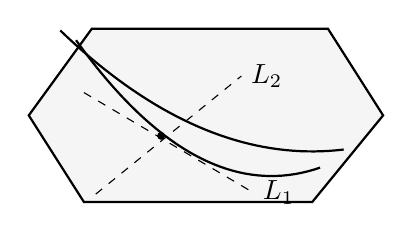
\begin{tikzpicture}[scale=1.0]
		% 曲面示意 (用椭圆表示)
		\draw[thick, fill=gray!8] (-2.1,0) -- (-1.3,1.1) -- (1.7,1.1) -- (2.4,0) -- (1.5,-1.1) -- (-1.4,-1.1) -- cycle;
		% 两条横截曲线
		\draw[thick] plot[domain=-1.7:1.9, samples=40] (\x, {0.15*\x*\x - 0.45*\x - 0.12});
		\draw[thick] plot[domain=-1.5:1.6, samples=40] (\x, {-0.5 - 0.55*\x + 0.28*\x*\x});
		% 交点与切线
		\fill (-0.42,-0.26) circle (0.05);
		\draw[dashed] (-1.4,0.29) -- (0.75,-0.98) node[right] {$L_1$};
		\draw[dashed] (-1.25,-1.0) -- (0.6,0.5) node[right] {$L_2$};
	\end{tikzpicture}
	\caption{曲面上横截的曲线}
	\label{fig:2.1}
\end{figure}

对子空间 $\Theta_{Y_i,x} \subset \Theta_{X,x}$ 用不等式 \eqref{eq:1.49} 与不等式 $\operatorname{codim} \Theta_{Y_i,x} \le \operatorname{codim}_X Y_i$, 可见 \eqref{eq:2.17} 蕴含等式
\[
	\dim \Theta_{Y_i,x} = \dim Y_i,
\]
即每个 $Y_i$ 在 $x$ 处非奇异; 还蕴含等式
\[
	\operatorname{codim}_{\Theta_{X,x}} \Bigl( \bigcap_{i=1}^{r} \Theta_{Y_i,x} \Bigr) = \sum_{i=1}^{r} \operatorname{codim} \Theta_{Y_i,x},
\]
即向量子空间 $\Theta_{Y_i,x} \subset \Theta_{X,x}$（在给定维数下交尽可能小这一意义上）横截. 由包含关系 $\bigcap_{i=1}^r \Theta_{Y_i,x} \supset \Theta_{Y,x}$（其中 $Y = \bigcap Y_i$）, 同样可推出 $Y$ 在 $x$ 处非奇异.

于是定理~\ref{thm:local-params-transversal} 断言子簇 $V(u_i)$ 横截.

设 $X'$ 是 $x$ 的使 $\bigcap X'_i = x = (0, \ldots, 0)$ 的仿射邻域. 若 $X' \subset \A^N$ 而 $t_i$ 是 $\A^N$ 的坐标, 则 $x$ 由 $t_1 = \cdots = t_N = 0$ 定义, 而 $\bigcap X'_i$ 在 $X'$ 中由 $u_1 = \cdots = u_n = 0$ 定义. 由 Nullstellensatz 得, 对某个 $k > 0$ 有 $(t_1, \ldots, t_N)^k \subset (u_1, \ldots, u_n)$, 这里 $(t_1, \ldots, t_N)$ 与 $(u_1, \ldots, u_n)$ 表示 $k[X']$ 中的理想. 对 $\mathcal O_x$ 中的理想 $(t_1, \ldots, t_N)$ 与 $(u_1, \ldots, u_n)$ 更是如此. 注意 $(t_1, \ldots, t_N) = \mathfrak m_x$, 故 $\mathfrak m_x^k \subset (u_1, \ldots, u_n)$. 事实上更强的结论成立.

\begin{theorem}\label{thm:params-generate}
	$x$ 处的局部参数生成 $\mathcal O_x$ 的极大理想 $\mathfrak m_x$.
\end{theorem}

\begin{proof}
	这是 Nakayama 引理（原书附录命题 A.11）作用于作为 $\mathcal O_x$-模的极大理想 $\mathfrak m_x$ 的直接推论. 由 §1.1 的引理, $\mathfrak m_x$ 是有限 $\mathcal O_x$-模. 既然局部参数生成 $\mathfrak m_x/\mathfrak m_x^2$, 由 Nakayama 引理它们生成 $\mathfrak m_x$. 定理证毕.
\end{proof}

\begin{example}[自由作用的商]\label{exam:quotient-nonsingular}
	设 $X$ 是非奇异仿射簇, $G$ 是 $X$ 的自同构的有限群, 如例~\ref{exam:quotient}. 设 $G$ 自由作用于 $X$, 即由 $g(x) = x$（$g \in G$, $x \in X$）可推出 $g = e$（$e$ 为恒等映射）. 我们证明在这些假设下商簇 $X/G$ 仍是非奇异的.

	设 $f: X \to Y = X/G$ 是例~\ref{exam:quotient} 构造的商映射, $n = \dim X = \dim Y$. 取 $x \in X$, 令 $y = f(x) \in Y$, 取 $x$ 处的局部参数 $u_1, \ldots, u_n$ 且 $u_i \in k[X]$, 则 $u_1, \ldots, u_n$ 生成 $\mathfrak m_x$. 对每个 $u_i$, 构造函数 $\bar u_i \in k[X]$, 使 $\bar u_i \equiv u_i \bmod \mathfrak m_x^2$, 且对一切 $g \ne e$ 有 $\bar u_i \in \mathfrak m_{g(x)}^2$. 为此只需把 $u_i$ 乘以一个元素 $h \in k[X]$ 的平方, 其中 $h(x) = 1$ 而对一切 $g \ne e$ 有 $h(g(x)) = 0$.

	令 $v_i = S(\bar u_i)$, 其中平均算子 $S$ 如原书附录命题 A.6 与例~\ref{exam:quotient}. 既然 $g \ne e$ 时 $g^* \bar u_i \in \mathfrak m_x^2$, 有 $v_i \equiv \frac{1}{|G|} u_i \bmod \mathfrak m_x^2$, 故 $v_1, \ldots, v_n$ 是 $x$ 处的局部参数. 但 $v_i \in k[Y]$ 且 $v_i(y) = 0$. 我们证明 $\mathfrak m_y = (v_1, \ldots, v_n)$. 设 $h \in \mathfrak m_y \cap k[Y]$, 则 $f^*(h) \in \mathfrak m_x$ 且 $f^*(h) = \sum h_i v_i$. 对此应用算子 $S$, 由 $S(f^*(h)) = f^*(h)$ 与 $S(v_i) = v_i$ 得 $f^*(h) = \sum S(h_i)\, v_i$. 于是 $\dim \mathfrak m_y/\mathfrak m_y^2 \le n$, 从而 $y$ 非奇异.
\end{example}

值得指出, 点 $x$ 的非奇异性由局部环 $\mathcal O_x$ 的纯代数性质刻画. 按定义, $x \in X$ 非奇异当且仅当 $\dim_k \mathfrak m_x/\mathfrak m_x^2 = \dim_x X$. 等式左端对任何 Noether 局部环 $\mathcal O$ 都有定义; 右端也可表述为局部环 $\mathcal O_x$ 的性质. 事实上, 由定理~\ref{thm:all-components} 与推论~\ref{cor:subvariety-dims}, $X$ 在 $x$ 处的维数可定义为使存在 $r$ 个函数 $u_1, \ldots, u_r \in \mathfrak m_x$ 且在 $x$ 的某邻域中由 $u_1 = \cdots = u_r = 0$ 定义的集合恰为 $x$ 的最小 $r$. 由 Nullstellensatz, 这一性质等价于对某个 $k > 0$ 有 $(u_1, \ldots, u_r) \supset \mathfrak m_x^k$.

对极大理想为 $\mathfrak m$ 的任意 Noether 局部环 $\mathcal O$, 使存在 $r$ 个函数 $u_1, \ldots, u_r \in \mathfrak m$ 且对某个 $k > 0$ 有 $(u_1, \ldots, u_r) \supset \mathfrak m^k$ 的最小数 $r$ 称为 $\mathcal O$ 的维数, 记作 $\dim \mathcal O$. 由 Nakayama 引理, 理想 $\mathfrak m$ 本身可由 $n$ 个元素生成, 其中 $n = \dim_{\mathcal O/\mathfrak m}(\mathfrak m/\mathfrak m^2)$, 故
\[
	\dim \mathcal O \le \dim_{\mathcal O/\mathfrak m} (\mathfrak m/\mathfrak m^2).
\]
若 $\dim \mathcal O = \dim_{\mathcal O/\mathfrak m}(\mathfrak m/\mathfrak m^2)$, 就称局部环 $\mathcal O$ 为\emph{正则}的. 于是 $x$ 是非奇异点当且仅当局部环 $\mathcal O_x$ 正则. 这就是点的非奇异性的代数含义.

\subsection{幂级数展开}

把幂级数与局部环 $\mathcal O_x$ 的元素联系起来的想法基于如下论证. 对任何函数 $f \in \mathcal O_x$, 令 $f(x) = \alpha_0$, $f_1 = f - \alpha_0$; 则 $f_1 \in \mathfrak m_x$. 设 $u_1, \ldots, u_n$ 是 $x$ 处的一组局部参数. 按定义, $u_1, \ldots, u_n$ 生成整个向量空间 $\mathfrak m_x/\mathfrak m_x^2$, 故存在 $\alpha_1, \ldots, \alpha_n \in k$ 使 $f_1 - \sum_{i=1}^n \alpha_i u_i \in \mathfrak m_x^2$. 令 $f_2 = f_1 - \sum \alpha_i u_i = f - \alpha_0 - \sum \alpha_i u_i$. 既然 $f_2 \in \mathfrak m_x^2$, 可写 $f_2 = \sum g_j h_j$, 诸 $g_j, h_j \in \mathfrak m_x$. 同上, 存在 $\beta_{ji}, \gamma_{ji} \in k$ 使
\[
	g_j - \sum_{i=1}^{n} \beta_{ji} u_i \in \mathfrak m_x^2, \qquad h_j - \sum_{i=1}^{n} \gamma_{ji} u_i \in \mathfrak m_x^2.
\]
令 $\sum_j \bigl( \sum_i \beta_{ji} u_i \bigr)\bigl( \sum_i \gamma_{ji} u_i \bigr) = \sum_{l,k=1}^{n} \alpha_{lk}\, u_l u_k$, 则 $f_2 - \sum \alpha_{lk} u_l u_k \in \mathfrak m_x^3$, 因此 $f_3 = f - \alpha_0 - \sum \alpha_i u_i - \sum \alpha_{lk} u_l u_k \in \mathfrak m_x^3$. 如此继续, 显然可找到型 $F_i \in k[T_1, \ldots, T_n]$（$\deg F_i = i$）使
\[
	f - \sum_{i=0}^{k} F_i(u_1, \ldots, u_n) \in \mathfrak m_x^{k+1}.
\]

\begin{definition}[形式幂级数环]\label{def:power-series-ring}
	变量 $(T_1, \ldots, T_n) = T$ 的\emph{形式幂级数环}是这样的环: 其元素为形如
	\begin{equation}
		\label{eq:2.18}
		\Phi = F_0 + F_1 + F_2 + \cdots
	\end{equation}
	的无穷表达式, 其中 $F_i \in k[T]$ 是 $i$ 次型; 环运算按下述规则定义: 若 $\Psi = G_0 + G_1 + G_2 + \cdots$, 则
	\[
		\Phi + \Psi = (F_0 + G_0) + (F_1 + G_1) + (F_2 + G_2) + \cdots,
	\]
	而 $\Phi\Psi = H_0 + H_1 + H_2 + \cdots$, 其中 $H_i = \sum_{j+l=i} G_j F_l$.
\end{definition}

形式幂级数环记作 $k[[T]]$. 它包含 $k$, 即 $i > 0$ 时 $F_i = 0$ 的幂级数. 若 $i$ 是使 $F_i \ne 0$ 的第一个下标, 则称 $F_i$ 为 \eqref{eq:2.18} 的首项. 乘积的首项等于首项之积, 故 $k[[T]]$ 没有零因子.

上面讨论的论证使我们可以给每个函数 $f \in \mathcal O_x$ 联系一个幂级数 $\Phi = F_0 + F_1 + F_2 + \cdots$. 于是得到如下定义.

\begin{definition}[Taylor 级数]\label{def:taylor-series}
	形式幂级数 $\Phi$ 称为函数 $f \in \mathcal O_x$ 的\emph{Taylor 级数}, 如果对每个 $k \ge 0$ 有
	\begin{equation}
		\label{eq:2.19}
		f - S_k(u_1, \ldots, u_n) \in \mathfrak m_x^{k+1}, \qquad S_k = \sum_{i=0}^{k} F_i.
	\end{equation}
\end{definition}

\begin{example}\label{exam:taylor-A1}
	设 $X = \A^1$, 坐标为 $t$, $x$ 是点 $t = 0$. 于是 $\mathfrak m_x = (t)$, 且可以给任何有理函数 $f(t) = P(t)/Q(t)$（$Q(0) \ne 0$）联系幂级数 $\sum_{m=0}^{\infty} \alpha_m t^m$, 使
	\[
		\frac{P(t)}{Q(t)} - \sum_{m=0}^{k} \alpha_m t^m \equiv 0 \bmod t^{k+1},
		\qquad\text{即}\qquad
		P(t) - Q(t) \sum_{m=0}^{k} \alpha_m t^m \equiv 0 \bmod t^{k+1}.
	\]
	这就是用待定系数法求有理函数幂级数系数的通常程序. 例如
	\[
		\frac{1}{1-t} = \sum_{m=0}^{\infty} t^m, \quad\text{因为}\quad \frac{1}{1-t} - \sum_{m=0}^{k} t^m = \frac{t^{k+1}}{1-t} \equiv 0 \bmod t^{k+1}.
	\]
	对应 $f \mapsto \Phi$ 实质上依赖于局部参数组 $u_1, \ldots, u_n$ 的选取.
\end{example}

刚才给出的论证证明了下面的断言.

\begin{theorem}\label{thm:taylor-exists}
	每个函数至少有一个 Taylor 级数.
\end{theorem}

到目前为止我们实质上没有用到 $x$ 非奇异, 只用到 $u_1, \ldots, u_n$ 生成 $\mathfrak m_x/\mathfrak m_x^2$. 现在使用 $x$ 的非奇异性.

\begin{theorem}\label{thm:taylor-unique}
	若 $x$ 非奇异, 则函数的 Taylor 级数唯一.
\end{theorem}

\begin{proof}
	显然只需证明函数 $f = 0$ 的任何 Taylor 级数都等于 $0$. 由 \eqref{eq:2.19}, 这等价于断言: 若 $u_1, \ldots, u_n$ 是非奇异点 $x$ 的局部参数, 则对 $k$ 次型 $F_k(T_1, \ldots, T_n)$,
	\begin{equation}
		\label{eq:2.20}
		F_k(u_1, \ldots, u_n) \in \mathfrak m_x^{k+1} \implies F_k(T_1, \ldots, T_n) = 0.
	\end{equation}
	设不然. 经非退化线性变换, 可使 $F_k$ 中 $T_n^k$ 的系数非零. 事实上, 该系数等于 $F_k(0, \ldots, 0, 1)$, 而若 $F_k(\alpha_1, \ldots, \alpha_n) \ne 0$（既然 $F_k \ne 0$, 这样的 $\alpha_1, \ldots, \alpha_n$ 当然存在）, 只需施行把向量 $(\alpha_1, \ldots, \alpha_n)$ 变到 $(0, \ldots, 0, 1)$ 的线性变换. 于是可设
	\[
		F_k(T_1, \ldots, T_n) = \alpha\, T_n^k + G_1(T_1, \ldots, T_{n-1})\, T_n^{k-1} + \cdots + G_k(T_1, \ldots, T_{n-1}),
	\]
	其中 $\alpha \ne 0$, 诸 $G_i$ 是 $T_1, \ldots, T_{n-1}$ 的 $i$ 次型.

	由定理~\ref{thm:params-generate} 容易推出, $\mathfrak m_x^{k+1}$ 的任何元素都可写成系数在 $\mathfrak m_x$ 中的 $u_1, \ldots, u_n$ 的 $k$ 次型. 于是 \eqref{eq:2.20} 左端可表为
	\begin{equation}
		\label{eq:2.21}
		\begin{split}
			\alpha\, u_n^k + G_1&(u_1, \ldots, u_{n-1})\, u_n^{k-1} + \cdots + G_k(u_1, \ldots, u_{n-1}) \\
			={}& \mu\, u_n^k + H_1(u_1, \ldots, u_{n-1})\, u_n^{k-1} + \cdots + H_k(u_1, \ldots, u_{n-1}),
		\end{split}
	\end{equation}
	其中 $\mu \in \mathfrak m_x$, 诸 $H_i$ 是 $i$ 次型. 由此得 $(\alpha - \mu)\, u_n^k \in (u_1, \ldots, u_{n-1})$. 既然 $\alpha \ne 0$, 有 $\alpha - \mu \notin \mathfrak m_x$ 而 $(\alpha - \mu)^{-1} \in \mathcal O_x$, 故 $u_n^k \in (u_1, \ldots, u_{n-1})$.

	于是 $V(u_n) \supset V(u_1) \cap \cdots \cap V(u_{n-1})$, 从而 $\Theta_n \supset \Theta_1 \cap \cdots \cap \Theta_{n-1}$（$\Theta_i$ 是 $V(u_i)$ 在 $x$ 处的切空间）, 故 $\Theta_1 \cap \cdots \cap \Theta_n = \Theta_1 \cap \cdots \cap \Theta_{n-1}$, 于是 $\dim \Theta_1 \cap \cdots \cap \Theta_n \ge 1$, 与定理~\ref{thm:local-params-transversal} 矛盾. 定理证毕.
\end{proof}

于是我们得到一个唯一确定的映射 $\tau: \mathcal O_x \to k[[T]]$, 把每个函数送到它的 Taylor 级数. 基于 $\tau$ 的定义 \eqref{eq:2.19} 的简单验证表明它是同态, 验证留给读者.

$\tau$ 的核是什么? 若对函数 $f \in \mathcal O_x$ 有 $\tau(f) = 0$, 则由 \eqref{eq:2.19} 这意味着对一切 $k$ 有 $f \in \mathfrak m_x^{k+1}$, 换言之 $f \in \bigcap_{k=0}^{\infty} \mathfrak m_x^k$. 于是我们讨论的是分析中在某点各阶导数全为 $0$ 的函数的类似物. 在我们的情形这样的函数必为 $0$, 这由原书附录命题 A.12 与 §1.1 的引理得出.

作为推论我们得到下面的结果.

\begin{theorem}\label{thm:taylor-injective}
	函数 $f \in \mathcal O_x$ 由它的任何 Taylor 级数唯一确定. 换言之, $\tau$ 是局部环 $\mathcal O_x$ 到形式幂级数环 $k[[T]]$ 的同构嵌入.
\end{theorem}

注意, 本节至今没有用到簇 $X$ 的不可约性. 反过来, 定理~\ref{thm:taylor-injective} 使我们可以对不可约性作出某些推断.

\begin{theorem}\label{thm:unique-component}
	若 $x$ 是 $X$ 的非奇异点, 则经过 $x$ 的 $X$ 的分支只有一个.
\end{theorem}

\begin{proof}
	把 $X$ 换成含于 $X' = X \setminus \bigcup Z_i$ 的 $x$ 的仿射邻域 $U$, 其中诸 $Z_i$ 是 $X$ 的不经过 $x$ 的分支. 那么 $k[U] \subset \mathcal O_x$. 由定理~\ref{thm:taylor-injective}, $\mathcal O_x$ 同构于形式幂级数环 $k[[T]]$ 的子环. 既然 $k[[T]]$ 没有零因子, 同构于其子环的 $k[U]$ 也没有. 故 $U$ 不可约, 即定理所断言. 定理证毕.
\end{proof}

\begin{corollary}\label{cor:singular-closed}
	代数簇 $X$ 的奇异点集是闭集.
\end{corollary}

\begin{proof}
	设 $X = \bigcup X_i$ 是不可约分解. 由定理~\ref{thm:unique-component}, $X$ 的奇异点集是诸 $X_i \cap X_j$（$i \ne j$）与诸 $X_i$ 的奇异点集之并; 作为有限多个闭集之并, 它是闭集. 推论证毕.
\end{proof}

若 $x$ 是奇异点, 我们至多只能把元素 $f \in \mathcal O_x$ 送到剩余类序列 $\xi_n = f + \mathfrak m_x^n \in \mathcal O_x/\mathfrak m_x^n$. 该序列有如下相容性: 若 $\theta_{n+1}: \mathcal O_x/\mathfrak m_x^{n+1} \to \mathcal O_x/\mathfrak m_x^n$ 是商映射, 则 $\theta_{n+1}(\xi_{n+1}) = \xi_n$. 全部这样的相容序列 $\{\xi_n\}$ 按分量加法与乘法组成一个环 $\widehat{\mathcal O}_x$, 称为 $\mathcal O_x$ 的\emph{完备化}.

我们刚定义了同态 $\tau: \mathcal O_x \to \widehat{\mathcal O}_x$, $\tau(f) = \{\xi_n\}$, $\xi_n = f + \mathfrak m_x^n$. 与非奇异点情形同样的论证表明 $\tau$ 是单射. 环 $\widehat{\mathcal O}_x$ 是局部的, 其极大理想 $\mathfrak M$ 由满足 $\xi_n \in \mathfrak m_x$ 的相容序列 $\{\xi_n\}$ 组成. 可以证明, 对 $\widehat{\mathcal O}_x$ 再施行同一构造不会得到新东西, 即 $(\widehat{\mathcal O}_x)\widehat{} = \widehat{\mathcal O}_x$, 且此时 $\tau$ 是同构.

若 $x$ 非奇异, 则 $\widehat{\mathcal O}_x$ 就是形式幂级数环. 一般地, $\widehat{\mathcal O}_x$ 是奇异点的重要特征: 若对 $x \in X$ 与 $y \in Y$ 完备局部环 $\widehat{\mathcal O}_x$ 与 $\widehat{\mathcal O}_y$ 同构, 就称簇 $X$ 与 $Y$ 在这些点的邻域中形式解析等价. 既然 $n$ 维簇的非奇异点 $x$ 的局部环 $\widehat{\mathcal O}_x$ 同构于 $\A^n$ 的点 $x'$ 的局部环的完备化, 同维数一切簇的一切非奇异点都有形式解析等价的邻域. 比较 §3 习题 8--16.

\subsection{实域与复域上的簇}

设 $k = \R$ 或 $\CC$. 我们证明此时函数 $f \in \mathcal O_x$ 的形式 Taylor 级数对小的 $T_1, \ldots, T_n$ 收敛.

设 $X \subset \A^N$ 是簇, $\mathfrak A_X = (F_1, \ldots, F_m)$, $\dim_x X = n$. 若 $x \in X$ 是非奇异点, 则矩阵 $\bigl( \partial F_i/\partial T_j(x) \bigr)$ 的秩为 $N - n$. 设
\begin{equation}
	\label{eq:2.22}
	\det \Bigl| \frac{\partial F_i}{\partial T_j}(x) \Bigr|_{\substack{i = 1, \ldots, N-n \\ j = n+1, \ldots, N}} \ne 0,
\end{equation}
且 $x$ 是原点. 那么前 $n$ 个坐标在 $X$ 上的限制 $t_1, \ldots, t_n$ 构成 $X$ 在 $x$ 处的局部参数组. 用 $X'$ 表示由
\begin{equation}
	\label{eq:2.23}
	F_1 = \cdots = F_{N-n} = 0
\end{equation}
定义的簇的经过 $x$ 的全部分支之并. 由 \eqref{eq:2.22}, $X'$ 在 $x$ 处的切空间 $\Theta'$ 的维数等于 $n$; 由相交维数定理, $\dim_x X' \ge n$. 既然 $\dim \Theta' \ge \dim_x X'$, 得 $\dim_x X' = n$ 且 $x$ 是 $X'$ 的非奇异点. 由此并由定理~\ref{thm:unique-component} 得 $X'$ 不可约. 显然 $X' \supset X$, 故 $\dim X' = \dim X$ 蕴含 $X' = X$.

于是 $X$ 可在 $x$ 的某邻域中由满足 \eqref{eq:2.22} 的 $N - n$ 个方程 \eqref{eq:2.23} 定义. 由隐函数定理（例如见 Goursat \cite[第 IX 章 \S\S 187--190]{goursat1916} 或 Fleming \cite[\S 4.6]{fleming1977}）, 存在 $n$ 个变量 $T_1, \ldots, T_n$ 的幂级数组 $\Phi_1, \ldots, \Phi_{N-n}$ 与 $\varepsilon > 0$, 使 $\Phi_j(T_1, \ldots, T_n)$ 对一切 $|T_i| < \varepsilon$ 收敛, 且
\begin{equation}
	\label{eq:2.24}
	F_i\bigl( T_1, \ldots, T_n, \Phi_1(T), \ldots, \Phi_{N-n}(T) \bigr) = 0;
\end{equation}
而且幂级数 $\Phi_1, \ldots, \Phi_{N-n}$ 的系数由关系 \eqref{eq:2.24} 唯一确定.

另一方面, 设取 $t_1, \ldots, t_n$ 为局部参数, 则形式幂级数 $\tau(T_{n+1}), \ldots, \tau(T_N)$ 也满足 \eqref{eq:2.24}, 故必与 $\Phi_1, \ldots, \Phi_{N-n}$ 一致, 于是当 $|T_j| < \varepsilon$（$j = 1, \ldots, n$）时 $\tau(T_{n+1}), \ldots, \tau(T_N)$ 收敛.

任何函数 $f \in \mathcal O_x$ 可写成 $f = P/Q$ 的形式, 其中 $P = P(T_1, \ldots, T_n)$ 与 $Q = Q(T_1, \ldots, T_n)$ 是多项式且 $Q(x) \ne 0$; 于是
\[
	\tau(f) = \frac{P(\tau(T_1), \ldots, \tau(T_n))}{Q(\tau(T_1), \ldots, \tau(T_n))}.
\]
$\tau(f)$ 的收敛性由幂级数收敛性的标准定理得出.

同样可证: 若 $u_1, \ldots, u_n$ 是另一组局部参数, 则行列式 $\det \bigl| \partial \tau(u_i)/\partial T_j(0, \ldots, 0) \bigr|$ 非零, 而 $t_1, \ldots, t_n$ 关于局部参数组 $u_1, \ldots, u_n$ 的 Taylor 级数由反解级数 $\tau(u_i) = \Phi_i(T_1, \ldots, T_n)$（$i = 1, \ldots, n$）得到, 故也有正收敛半径. 因此对 $f \in \mathcal O_x$, 无论取哪组局部参数, 级数 $\tau(f)$ 都有正收敛半径.

隐函数定理不仅断言收敛级数 $\Phi_1, \ldots, \Phi_{N-n}$ 存在, 而且断言存在 $\eta > 0$, 使满足 $|t_i| < \eta$（$i = 1, \ldots, N$）的任何点 $(t_1, \ldots, t_N) \in X$ 都形如 $t_{n+i} = \Phi_i(t_1, \ldots, t_n)$（$i = 1, \ldots, N-n$）. 由此可知 $(t_1, \ldots, t_N) \mapsto (t_1, \ldots, t_n)$ 是集合 $\{\, (t_1, \ldots, t_N) \in X \mid |t_i| < \eta \,\}$ 到 $n$ 维空间中某区域的双射同胚.

既然在我们的情形 $k = \R$ 或 $\CC$, $k$ 上的射影空间 $\PP^N$ 是拓扑空间, 代数簇 $X \subset \PP^N$ 也是拓扑空间. 分别在 $k = \R$ 或 $\CC$ 的情形, $X$ 上的这个拓扑称为 $X$ 的实拓扑或复拓扑. 这个拓扑及由它导出的概念, 不应与至今使用的具有拓扑字面的术语（闭集, 邻域, 开集, 闭包等）相混淆.

前面的论证表明: 对 $n$ 维簇 $X$, 任何非奇异点在实拓扑中有一个同胚于 $\R^n$ 中某区域的邻域. 故若 $X$ 的每点都非奇异, 则 $X$ 是拓扑意义上的 $n$ 维流形. 若 $k = \CC$, 非奇异点 $x \in X$ 在复拓扑中有同胚于 $n$ 维复空间 $\CC^n$ 中某区域的邻域, 从而同胚于 $\R^{2n}$ 中某区域. 因此若 $X$ 的一切点都非奇异, 则 $X$ 是 $2n$ 维流形.

容易证明, $k = \R$ 或 $\CC$ 时 $\PP^N$ 在实拓扑或复拓扑中是紧的, 于是射影簇 $X$ 是紧的. 若 $k = \CC$, 反之亦然: 复拓扑中紧的拟投影簇是射影簇（见原书第 7 章第 2.6 节习题 2）.

最后指出, 本节所述一切（上一段除外）都可逐字逐句地搬到 $k$ 是 $p$ 进数域的情形.

\subsection{第 2 节习题}

\begin{compactenum}
	\item 证明: 对 $n$ 维簇 $X$, 使给定的 $n$ 个函数不构成局部参数组的点集是闭集.
	\item 证明: 多项式 $f \in k[T] = k[\A^1]$ 在点 $T = \alpha$ 处是局部参数, 当且仅当 $\alpha$ 是 $f$ 的单根.
	\item 证明: 形式幂级数 $\Phi = F_0 + F_1 + \cdots$ 在 $k[[T]]$ 中可逆, 当且仅当 $F_0 \ne 0$.
	\item 设 $T$ 是未定元. 考虑形如 $\alpha_{-n} T^{-n} + \alpha_{-n+1} T^{-n+1} + \cdots + \alpha_0 + \alpha_1 T + \cdots$ 的表达式组成的环 $k((T))$. 证明 $k((T))$ 是域, 且同构于 $k[[T]]$ 的分式域.（它称为形式 Laurent 级数域.）
	\item 设 $S \subset \A^2$ 是由 $X^2 + Y^2 = 1$ 给出的圆, 基域 $k$ 特征为 $0$. 证明 $X$ 在 $x = (0,1)$ 处是局部参数, 且 $Y$ 的 Taylor 展开为
	\[
		\tau(Y) = \sum_{n=0}^{\infty} \frac{(-1)^n\, (1/2)(1/2 - 1) \cdots (1/2 - n + 1)}{n!}\, X^{2n}.
	\]
	\item 证明: 若 $x$ 是奇异点, 则任何函数 $f \in \mathcal O_x$ 都有无穷多个不同的 Taylor 级数.
	\item 设 $X = \A^1$ 而 $x \in X$. 证明 $\tau(\mathcal O_x)$ 不是整个 $k[[T]]$.
\end{compactenum}

\section{非奇异点的性质}

\subsection{余维 \texorpdfstring{$1$}{1} 子簇}

局部环理论使我们能够证明非奇异簇的一个重要性质, 它是定理~\ref{thm:codim1-principal} 的类似物. 所讨论的问题是: 余维 $1$ 子簇 $Y \subset X$ 能否由单个方程定义. 对奇异簇, 这一性质一般不成立（比较推论~\ref{cor:thm121-fails}）; 但我们证明它在非奇异簇上局部成立. 为陈述结果, 引入如下定义.

\begin{definition}[局部方程]\label{def:local-equations}
	函数 $f_1, \ldots, f_m \in \mathcal O_x$ 称为子簇 $Y \subset X$ 在 $x$ 的某邻域中的\emph{局部方程}, 如果存在 $x$ 的仿射邻域 $X'$ 使 $f_1, \ldots, f_m \in k[X']$ 且在 $k[X']$ 中有 $\mathfrak a_{Y'} = (f_1, \ldots, f_m)$, 其中 $Y' = Y \cap X'$.
\end{definition}

用 $x$ 的局部环 $\mathcal O_x$ 的语言重述这一条件是方便的. 考虑由在 $x$ 的某邻域中在 $Y$ 上为零的函数 $f \in \mathcal O_x$ 组成的理想 $\mathfrak a_{Y,x} \subset \mathcal O_x$. 对仿射簇 $X$, 显然
\[
	\mathfrak a_{Y,x} = \{\, f = u/v \mid u, v \in k[X],\ u \in \mathfrak a_Y,\ v(x) \ne 0 \,\},
\]
而若 $Y$ 的全部分支都经过 $x$, 则 $\mathfrak a_Y = \mathfrak a_{Y,x} \cap k[X]$.

\begin{lemma}\label{lem:local-equations-ideal}
	函数 $f_1, \ldots, f_m \in \mathcal O_x$ 是 $Y$ 在 $x$ 的某邻域中的局部方程, 当且仅当 $\mathfrak a_{Y,x} = (f_1, \ldots, f_m)$.
\end{lemma}

\begin{proof}
	若在 $k[X]$ 中 $\mathfrak a_Y = (f_1, \ldots, f_m)$, 那么显然在 $\mathcal O_x$ 中也有 $\mathfrak a_{Y,x} = (f_1, \ldots, f_m)$. 反之, 设 $\mathfrak a_{Y,x} = (f_1, \ldots, f_m)$（诸 $f_i \in \mathcal O_x$）, 并设 $\mathfrak a_Y = (g_1, \ldots, g_s)$（诸 $g_i \in k[X]$）. 既然 $g_i \in \mathfrak a_{Y,x}$, 可写
	\begin{equation}
		\label{eq:2.25}
		g_i = \sum_{j=1}^{m} h_{ij} f_j, \qquad h_{ij} \in \mathcal O_x.
	\end{equation}
	函数 $f_i$ 与 $h_{ij}$ 都在 $x$ 的某个主开邻域 $U$ 中正则. 设 $U = X \setminus V(g)$（$g \in k[X]$）, 则 $k[U]$ 由形如 $u/g^l$（$u \in k[X]$, $l \ge 0$）的元素组成. 于是由 \eqref{eq:2.25}, 在 $k[U]$ 中有
	\[
		(g_1, \ldots, g_s) = \mathfrak a_Y\, k[U] \subset (f_1, \ldots, f_m).
	\]
	我们证明 $\mathfrak a_Y\, k[U] = \mathfrak a_{Y'}$（此时 $Y' = Y \cap U$）. 由此得 $\mathfrak a_{Y'} \subset (f_1, \ldots, f_m)$; 又 $f_i \in \mathfrak a_{Y'}$, 便得引理的断言.

	剩下证明 $\mathfrak a_Y\, k[U] = \mathfrak a_{Y'}$. 包含关系 $\mathfrak a_Y\, k[U] \subset \mathfrak a_{Y'}$ 是显然的. 设 $v \in \mathfrak a_{Y'}$, 则 $v = u/g^l$（$u \in k[X]$）, 于是 $u = v g^l$, 故 $u \in \mathfrak a_Y$; 又 $1/g^l \in k[U]$, 得 $v = u/g^l \in \mathfrak a_Y\, k[U]$. 引理证毕.
\end{proof}

我们的目标是证明下面的结果.

\begin{theorem}\label{thm:codim1-local-eq}
	余维 $1$ 的不可约子簇 $Y \subset X$ 在任何非奇异点 $x \in X$ 的某邻域中有局部方程.
\end{theorem}

证明完全循定理~\ref{thm:codim1-principal} 的步骤. 不过那里用到了 $k[T]$ 是唯一分解整环这一事实; 这里起 $k[T]$ 作用的是局部环 $\mathcal O_x$, 它具有类似的性质.

\begin{theorem}\label{thm:local-ufd}
	非奇异点的局部环 $\mathcal O_x$ 是唯一分解整环.
\end{theorem}

定理~\ref{thm:local-ufd} 的证明基于先建立幂级数环 $k[[T]]$ 是唯一分解整环. 这是一个相当初等的事实, 与多项式环的相应结果类似; 我们只指出证明的主要步骤. 完全初等的（不依赖本书其余部分的）证明见 Zariski--Samuel \cite[第 VII 章第 1 节定理 6]{zariski-samuel1960}.

称幂级数 $\Phi(T_1, \ldots, T_n)$ 关于变量 $T_n$ 是正则的, 如果它的首项型（设为 $m$ 次）含有项 $c_m T_n^m$（$c_m \ne 0$）. 变量 $T_1, \ldots, T_n$ 的线性变换显然诱导 $k[[T]]$ 的自同构; 特别地, 可施行线性变换使任何给定的非零幂级数 $\Phi$ 关于 $T_n$ 正则.

\begin{lemma}[Weierstrass 预备定理]\label{lem:weierstrass-prep}
	设幂级数 $\Phi \in k[[T]]$ 关于 $T_n$ 正则且首项型为 $m$ 次, 则存在常数项非零的幂级数 $U \in k[[T]]$, 使 $\Phi U$ 是系数在 $k[[T_1, \ldots, T_{n-1}]]$ 中的关于 $T_n$ 的多项式, 即
	\[
		\Phi U = T_n^m + R_1 T_n^{m-1} + \cdots + R_m, \qquad R_i = R_i(T_1, \ldots, T_{n-1}) \in k[[T_1, \ldots, T_{n-1}]].
	\]
	证明见 Zariski--Samuel \cite[第 VII 章第 1 节定理 5]{zariski-samuel1960}.
\end{lemma}

\begin{lemma}\label{lem:power-series-ufd}
	形式幂级数环 $k[[T]]$ 是唯一分解整环.
\end{lemma}

引理~\ref{lem:weierstrass-prep} 使我们可以对变量个数作归纳来证明这一断言, 把它归结为系数在 $k[[T_1, \ldots, T_{n-1}]]$ 中的 $T_n$ 的多项式的类似命题. 详细证明见 Zariski--Samuel \cite[第 VII 章第 1 节定理 6]{zariski-samuel1960}.

\begin{proof}[定理~\ref{thm:local-ufd} 的证明]
	用 $\widehat{\mathcal O}_x$ 表示形式幂级数环, 由定理~\ref{thm:taylor-injective} 可把 $\mathcal O_x$ 视为其子环 $\mathcal O_x \subset \widehat{\mathcal O}_x$. 用 $\widehat{\mathfrak m}_x$ 表示 $\widehat{\mathcal O}_x$ 中由常数项为 $0$ 的形式幂级数组成的理想, 则 $\widehat{\mathfrak m}_x^k$ 是不含次数 $< k$ 的项的形式幂级数组成的理想. 由嵌入 $\mathcal O_x \hookrightarrow \widehat{\mathcal O}_x$ 的定义（见 \eqref{eq:2.19}）得 $\widehat{\mathfrak m}_x^k \cap \mathcal O_x = \mathfrak m_x^k$. 于是原书附录命题 A.14 的条件满足, 它保证由 $\widehat{\mathcal O}_x$ 是唯一分解整环（引理~\ref{lem:power-series-ufd}）可推出 $\mathcal O_x$ 是唯一分解整环. 定理证毕.
\end{proof}

\begin{proof}[定理~\ref{thm:codim1-local-eq} 的证明]
	如前所述, 证明与定理~\ref{thm:codim1-principal} 完全相同. 既然断言是局部的, 可设 $X$ 仿射. 取任一在 $Y$ 上为零的函数 $f \in \mathcal O_x$, 把 $f$ 在 $\mathcal O_x$ 中分解为素因子之积. 由 $Y$ 的不可约性, 某个因子也在 $Y$ 上为零; 把它记作 $g$, 我们证明它是 $Y$ 的局部方程. 把 $X$ 换成更小的 $x$ 的仿射邻域, 可设 $g$ 在 $X$ 上正则.

	既然 $V(g) \supset Y$ 且二者都是余维 $1$ 子簇, 有 $V(g) = Y \cup Y'$. 若 $Y' \ni x$, 则存在函数 $h$ 与 $h'$, 使 $hh'$ 在 $V(g)$ 上为零而 $h$ 与 $h'$ 都不在 $V(g)$ 上为零. 于是对某个 $r$, 在 $k[X]$ 中 $g \mid (hh')^r$, 从而更加在 $\mathcal O_x$ 中 $g \mid (hh')^r$. 既然 $\mathcal O_x$ 是唯一分解整环, 由此得在 $\mathcal O_x$ 中 $g$ 整除 $h$ 或 $h'$. 于是 $h$ 或 $h'$ 在 $x$ 的某邻域中在 $V(g)$ 上为零, 从而（过渡到更小的邻域后）在整个 $V(g)$ 上为零, 与 $Y' \ni x$ 矛盾. 故 $Y' \not\ni x$; 再把 $X$ 换成足够小的 $x$ 的仿射邻域, 可设 $V(g) = Y$.

	现在若 $u$ 在 $Y$ 上为零, 则对某个 $s > 0$ 在 $k[X]$ 中 $g \mid u^s$, 从而更加在 $\mathcal O_x$ 中 $g \mid u^s$. 由此得在 $\mathcal O_x$ 中 $g \mid u$. 于是 $\mathfrak a_{Y,x} = (g)$, 定理证毕.
\end{proof}

定理~\ref{thm:codim1-local-eq} 有许多应用. 下面是第一个（比较第一章定理~\ref{thm:rational-map-regular}）.

\begin{theorem}\label{thm:rational-map-codim2}
	若 $X$ 是非奇异簇而 $\varphi: X \to \PP^n$ 是到射影空间的有理映射, 则 $\varphi$ 不正则的点集的余维数 $\ge 2$.
\end{theorem}

\begin{proof}
	回忆有理映射 $\varphi$ 的不正则点集（不定点轨迹）是闭集. 定理的断言是局部的, 只需在非奇异点 $x \in X$ 的邻域中证明. 可把 $\varphi$ 写成 $\varphi = (f_0 : \cdots : f_n)$（诸 $f_i \in k(X)$）, 且在不改变 $\varphi$ 的前提下通分, 使诸 $f_i \in \mathcal O_x$ 且在 $\mathcal O_x$ 中没有公因子. 此时 $\varphi$ 只在使 $f_0 = \cdots = f_n = 0$ 的点处不正则. 但没有余维 $1$ 子簇 $Y$ 能含于这些方程定义的集合中; 事实上, 由定理~\ref{thm:codim1-local-eq}, $\mathfrak a_{Y,x} = (g)$, 而诸 $f_i$ 在 $\mathcal O_x$ 中将以 $g$ 为公因子, 与假设矛盾. 定理证毕.
\end{proof}

\begin{corollary}\label{cor:curve-rational-regular}
	非奇异曲线到射影空间的任何有理映射都是正则的.
\end{corollary}

\begin{corollary}\label{cor:curves-birational-iso}
	双有理等价的非奇异射影曲线是同构的.
\end{corollary}

设 $k = \CC$ 是复数域. 由推论~\ref{cor:curves-birational-iso} 可知: 若两条曲线 $X'$ 与 $X''$ 双有理等价, 则 $X'$ 与 $X''$ 的复点集（带复拓扑）同胚. 事实上, 此时正则函数从而正则映射由收敛幂级数定义, 因而是连续的.

同样的结论对由实系数方程定义且存在定义在 $\R$ 上的双有理映射 $\varphi: X' \to X''$（即由实系数有理函数定义）的曲线的实点集成立. 这有时使我们能容易地推断两条曲线在 $\R$ 上不双有理等价. 例如, 由 $y^2 = x^3 - x$ 定义的曲线 $X$ 由两个连通分支组成（图~\ref{fig:2.2}）, 因此 $X$ 在 $\R$ 上不是有理的, 因为 $\PP^1$ 同胚于圆周, 只有一个连通分支.

用类似的思想可以证明曲线 $X$（$y^2 = x^3 - x$）在 $\CC$ 上也是非有理的. 为此需比较 $X$ 与 $\PP^1$ 的复点集（带复拓扑）并证明它们不同胚: 前者同胚于环面, 后者同胚于球面. 这是原书第 7 章第 3.3 节所证结果的特殊情形. 图~\ref{fig:2.3} 显示了 $X$ 的实点集作为其复点集的子集的样子.

\begin{figure}[htbp]
	\centering
	\begin{tikzpicture}[scale=1.1]
		\draw[->] (-1.6,0) -- (2.4,0) node[right] {$x$};
		\draw[->] (0,-2.0) -- (0,2.0) node[above] {$y$};
		% 有界分支 (卵形): x in [-1,0]
		\draw[thick] plot[domain=-1:0, samples=60] (\x, {sqrt(\x*\x*\x - \x)});
		\draw[thick] plot[domain=-1:0, samples=60] (\x, {-sqrt(\x*\x*\x - \x)});
		% 无界分支: x >= 1
		\draw[thick] plot[domain=1:2.1, samples=60] (\x, {sqrt(\x*\x*\x - \x)});
		\draw[thick] plot[domain=1:2.1, samples=60] (\x, {-sqrt(\x*\x*\x - \x)});
		\fill (-1,0) circle (0.035);
		\fill (0,0) circle (0.035);
		\fill (1,0) circle (0.035);
	\end{tikzpicture}
	\caption{$\R$ 上的 $y^2 = x^3 - x$}
	\label{fig:2.2}
\end{figure}

\begin{figure}[htbp]
	\centering
	\begin{tikzpicture}[scale=1.0]
		% 环面示意 (两圈椭圆)
		\draw[thick] (0,0) ellipse (2.2 and 0.85);
		\draw[thick] (0,0.25) ellipse (1.35 and 0.45);
		\fill[white] (0,0.25) ellipse (1.3 and 0.42);
		% 环面上的实点集: 两条闭曲线 (示意)
		\draw[thick, dashed] (-1.95,0.28) .. controls (-1.0,0.75) and (1.0,0.75) .. (1.95,0.28);
		\draw[thick, dashed] (-1.95,-0.28) .. controls (-1.0,-0.62) and (1.0,-0.62) .. (1.95,-0.28);
		\node[below] at (0,-1.15) {实点集（虚线）位于环面上};
	\end{tikzpicture}
	\caption{$\CC$ 上的 $y^2 = x^3 - x$}
	\label{fig:2.3}
\end{figure}

\subsection{非奇异子簇}

定理~\ref{thm:codim1-local-eq} 不能推广到余维数 $> 1$ 的子簇 $Y \subset X$（例如比较第一章 §6 习题 2）. 但对在 $x$ 处非奇异的子簇, 类似的结论成立. 我们证明一个略为精确的事实, 从一个辅助断言开始.

\begin{theorem}\label{thm:params-subvariety}
	设 $X$ 是仿射簇, $x \in X$ 是非奇异点, $u_1, \ldots, u_n$ 是 $X$ 上正则的函数且构成 $x$ 处的局部参数组. 那么对 $m \le n$, 由 $u_1 = \cdots = u_m = 0$ 定义的子簇 $Y$ 在 $x$ 处非奇异, 在 $x$ 的某仿射邻域中有 $\mathfrak a_Y = (u_1, \ldots, u_m)$, 且 $u_{m+1}, \ldots, u_n$ 构成 $Y$ 在 $x$ 处的局部参数组.
\end{theorem}

\begin{proof}
	对 $m$ 作归纳. 对 $m = 1$, 定理~\ref{thm:codim1-local-eq} 表明在 $x$ 的某仿射邻域中 $\mathfrak a_Y = (f)$. 设 $u_1 = f v$, 则 $d_x u_1 = v(x)\, d_x f$. 既然 $u_1$ 是局部参数组的元素, $d_x u_1 \ne 0$, 故 $v(x) \ne 0$, 于是在某个更小的开集中 $\mathfrak a_Y = (u_1)$. 又 $d_x u_1 \ne 0$ 推出 $x$ 是 $Y$ 的非奇异点.

	由 $\Theta_{X,x}$ 加上条件 $d_x u_1 = 0$ 显然得到切空间 $\Theta_{Y,x}$. 因此 $d_x u_2, \ldots, d_x u_n$ 构成 $\Theta_{Y,x}^*$ 的基, 即 $u_2, \ldots, u_n$ 是 $Y$ 在 $x$ 处的局部参数组.

	一般情形, 令 $X' \subset X$ 是由 $u_1 = 0$ 定义的子簇, 则 $Y \subset X'$ 在 $X'$ 中由方程 $u_2 = \cdots = u_m = 0$ 定义, 对 $m-1$ 用归纳即得. 定理证毕.
\end{proof}

现在证明在 $x$ 处非奇异的任何子簇 $Y \subset X$ 在 $x$ 的某邻域中可由定理~\ref{thm:params-subvariety} 所述的方式给出.

\begin{theorem}\label{thm:subvariety-local-params}
	设 $X$ 是簇, $Y \subset X$ 是子簇, $x \in Y$ 是 $X$ 与 $Y$ 的公共非奇异点. 那么可以选取 $X$ 在 $x$ 处的局部参数组 $u_1, \ldots, u_n$ 与 $x$ 的仿射邻域 $U$, 使在 $U$ 中 $\mathfrak a_Y = (u_1, \ldots, u_m)$.
\end{theorem}

在特殊情形 $X = \A^n$ 而 $k = \R$ 或 $\CC$, 类似的事实已在 §2.3 证明.

\begin{proof}
	切空间的包含 $\Theta_{Y,x} \hookrightarrow \Theta_{X,x}$ 对应对偶空间的满射 $\varphi: \mathfrak m_{X,x}/\mathfrak m_{X,x}^2 \to \mathfrak m_{Y,x}/\mathfrak m_{Y,x}^2$（由函数从 $X$ 限制到 $Y$ 定义）. 可以选取 $\mathfrak m_{X,x}/\mathfrak m_{X,x}^2$ 的基 $u_1, \ldots, u_n$, 使 $u_1, \ldots, u_m \in \mathfrak a_Y$ 而 $u_{m+1}, \ldots, u_n$ 在 $Y$ 上的限制构成 $\mathfrak m_{Y,x}/\mathfrak m_{Y,x}^2$ 的基. 取使诸 $u_i$ 都正则的 $x$ 的仿射邻域, 在其中考虑由 $u_1 = \cdots = u_m = 0$ 定义的子簇 $Y'$. 由构造 $Y' \supset Y$. 我们证明 $Y = Y'$, 于是断言由定理~\ref{thm:params-subvariety} 得出.

	由定理~\ref{thm:params-subvariety}, $Y'$ 在 $x$ 处非奇异, 由定理~\ref{thm:unique-component} 在 $x$ 的某邻域中不可约, 且 $\dim Y' = n - m$. 由构造显然 $\dim \Theta_{Y,x} = n - m$. 故 $Y = Y'$; 又由定理~\ref{thm:params-subvariety} 有 $\mathfrak a_{Y'} = (u_1, \ldots, u_m)$, 于是在 $x$ 的某邻域中也有 $\mathfrak a_Y = (u_1, \ldots, u_m)$. 定理证毕.
\end{proof}

\subsection{第 3 节习题}

\begin{compactenum}
	\item 证明: 若 $t$ 是代数曲线非奇异点处的局部参数, 则任何函数 $f \in \mathcal O_x$ 都可唯一地写成 $f = t^n u$ 的形式, 其中 $n \ge 0$, $u$ 是 $\mathcal O_x$ 的可逆元. 由此推出定理~\ref{thm:local-ufd} 对曲线的情形成.
	\item 证明定理~\ref{thm:local-params-transversal} 的逆: 若余维 $1$ 子簇 $D_1, \ldots, D_n$ 在 $x$ 处横截相交, 而 $u_1, \ldots, u_n$ 是它们在 $x$ 的某邻域中的局部方程, 则 $u_1, \ldots, u_n$ 构成 $x$ 处的局部参数组.
	\item 没有非奇异性假设时推论~\ref{cor:curves-birational-iso} 是否成立? 定理~\ref{thm:rational-map-codim2} 本身呢?
	\item 证明: 代数曲线 $X$ 的点 $x$ 非奇异, 当且仅当 $x$ 在 $X$ 上有局部方程.
	\item 设 $X \subset \A^3$ 是由 $x^2 + y^2 - z^2$ 给出的锥面. 证明母线 $L$（由 $x = 0$, $y = z$ 定义）在 $(0,0,0)$ 的任何邻域中没有局部方程.
	\item 设 $\varphi: \PP^2 \to \PP^2$ 是由 $\varphi(x_0 : x_1 : x_2) = (x_1 x_2 : x_0 x_2 : x_0 x_1)$ 定义的有理映射. 考虑点 $x = (1 : 0 : 0)$ 与在 $x$ 处非奇异的曲线 $C \subset \PP^2$. 由定理~\ref{thm:rational-map-codim2}, $\varphi$ 在 $C$ 上的限制在 $x$ 处正则, 因此把 $x$ 映到某点, 记作 $\varphi_C(x)$. 证明 $\varphi_{C_1}(x) = \varphi_{C_2}(x)$ 当且仅当 $C_1$ 与 $C_2$ 在 $x$ 处相切, 即 $\Theta_{C_1,x} = \Theta_{C_2,x}$.
	\item 证明: 若 $\varphi = f/g$ 是有理函数, $f$ 与 $g$ 在非奇异点 $x$ 处正则, 且幂级数 $\tau(f)$ 被 $\tau(g)$ 整除, 则 $\varphi$ 在 $x$ 处正则.（提示: 利用原书附录命题 A.14 的论证.）
	\item 下述断言将在后面的习题中使用. 设 $X \subset \A^n$ 是仿射簇, $x \in X$, $\mathfrak a_X = (f_1, \ldots, f_m)$. 证明
	\[
		\widehat{\mathcal O}_x = k[[T_1, \ldots, T_n]]/\bar{\mathfrak a}_X, \qquad \bar{\mathfrak a}_X = (\tau(f_1), \ldots, \tau(f_m)),
	\]
	其中 $\tau(f_i)$ 是 $f_i$ 如 §2.2 的 Taylor 级数.（提示: 利用 Atiyah--Macdonald \cite[第 10 章]{atiyah-macdonald1969} 的结果.）
	\item 证明: $\A^n$ 与自身的形式解析等价（即形式解析自同构）在 $0$ 的邻域中由无常数项且线性项构成的行列式非零的幂级数 $\Phi_1, \ldots, \Phi_n$ 给出.
	\item 证明: 过原点 $0 \in \A^2$ 的两条方程为 $F = 0$ 与 $G = 0$ 的平面曲线在 $0$ 的邻域中形式解析等价, 当且仅当存在 $\A^2$ 的由幂级数 $\Phi_1, \Phi_2$ 给出的形式解析自同构, 使 $F(\Phi_1, \Phi_2) = G U$, 其中 $U$ 是常数项非零的幂级数.
	\item 证明: 以 $0$ 为具有两条不同切线的二重点的任何非奇异代数曲线, 在 $0$ 的邻域中形式解析等价于曲线 $xy = 0$.（提示: 利用习题 10, 在理想 $(x,y)$ 的越来越高次幂模掉的意义下寻找 $\Phi_1, \Phi_2$.）
	\item 在特征 $0$ 的域上按形式解析等价对代数平面曲线的二重点分类.
	\item 设 $X$ 是 $\A^n$ 中方程为 $F = F_2(T) + F_3(T) + \cdots + F_k(T) = 0$ 的超曲面, 其中 $F_2(T)$ 是秩极大的二次型. 证明: $X$ 在 $0$ 的邻域中形式解析等价于二次锥面 $T_1^2 + \cdots + T_n^2 = 0$.
	\item 构造无穷多条非奇异射影曲线, 使其中任何两条在 $\R$ 上不同构.
	\item 设非奇异不可约 $n$ 维仿射簇 $X \subset \A^n$ 由方程 $F_1 = \cdots = F_m = 0$ 给出, 且对每点 $x = (x_1, \ldots, x_n) \in X$, 由 $\sum (\partial F_i/\partial T_j)(x)(T_j - x_j) = 0$ 定义的空间是 $n$ 维的. 证明此时 $\mathfrak a_X = (F_1, \ldots, F_m)$.
	\item 从习题 15 推出: 若把 Grassmann 簇 $\operatorname{Grass}(2, r)$ 的 Plücker 方程 $x \wedge x = 0$ 写成 $F_1 = \cdots = F_m = 0$, 则 $F_1, \ldots, F_m$ 生成 $\operatorname{Grass}(2, r)$ 的理想.（比较例~\ref{exam:grassmannian} 与例~\ref{exam:tangent-grassmann} 后的注记.）
\end{compactenum}

\section{双有理映射的结构}

\subsection{射影空间中的胀开}

前一节我们证明了非奇异射影曲线之间的双有理映射是同构（定理~\ref{thm:rational-map-codim2}, 推论~\ref{cor:curves-birational-iso}）. 这对高维簇不再成立. 例如, 球极投影建立非奇异二次曲面 $Q \subset \PP^3$ 与射影平面 $\PP^2$ 之间的双有理等价, 但它不是正则映射（见第一章 §4 习题 7, 并比较第一章的命题~\ref{prop:common-zero} 与推论~\ref{cor:r-forms}）. 本节定义并研究最简单且最典型的非同构双有理映射: 胀开.

考虑两个射影空间: 齐次坐标为 $x_0, \ldots, x_n$ 的 $\PP^n$ 与齐次坐标为 $y_1, \ldots, y_n$ 的 $\PP^{n-1}$. 对点 $x = (x_0 : \cdots : x_n) \in \PP^n$ 与 $y = (y_1 : \cdots : y_n) \in \PP^{n-1}$, 把积 $\PP^n \times \PP^{n-1}$ 中的点 $(x, y)$ 也记作 $(x_0 : \cdots : x_n;\, y_1 : \cdots : y_n)$. 考虑由方程
\begin{equation}
	\label{eq:2.26}
	x_i\, y_j = x_j\, y_i \qquad (i, j = 1, \ldots, n)
\end{equation}
定义的闭子簇 $\Pi \subset \PP^n \times \PP^{n-1}$.

\begin{definition}[胀开]\label{def:blowup}
	限制第一投影 $\PP^n \times \PP^{n-1} \to \PP^n$ 得到的映射 $\sigma: \Pi \to \PP^n$ 称为以 $\xi$ 为中心的\emph{胀开}\index{zhangkai@胀开}\footnote{这一概念在文献中还有许多名称: $\sigma$-过程, 单项变换, 膨胀, 二次变换等.}.
\end{definition}

用 $\xi$ 表示点 $\xi = (1 : 0 : \cdots : 0) \in \PP^n$. 若 $(x_0 : \cdots : x_n) \ne \xi$, 则由 \eqref{eq:2.26} 得 $(y_1 : \cdots : y_n) = (x_1 : \cdots : x_n)$, 于是由
\begin{equation}
	\label{eq:2.27}
	(x_0 : \cdots : x_n) \mapsto \bigl( (x_0 : \cdots : x_n),\ (x_1 : \cdots : x_n) \bigr)
\end{equation}
定义的映射 $\sigma^{-1}: \PP^n \setminus \xi \to \Pi$ 是 $\sigma$ 的逆. 然而当 $(x_0 : \cdots : x_n) = \xi$ 时, \eqref{eq:2.26} 对诸 $y_i$ 的任何取值都满足. 于是 $\sigma^{-1}(\xi) = \xi \times \PP^{n-1}$, 而 $\sigma$ 给出 $\PP^n \setminus \xi$ 与 $\Pi \setminus (\xi \times \PP^{n-1})$ 之间的同构. 点 $\xi$ 称为胀开 $\sigma$ 的中心.

我们来描述 $\Pi$ 在形如 $(\xi;\, y_1, \ldots, y_n)$ 的点的邻域中的结构. 某个 $y_i \ne 0$, 于是该点含于由 $x_0 \ne 0$, $y_i \ne 0$ 定义的 $\Pi$ 的开集 $U_i$; 在 $U_i$ 中甚至可设 $x_0 = 1$, $y_i = 1$. 此时 \eqref{eq:2.26} 取形式 $x_j = y_j x_i$（$j = 1, \ldots, n$, $j \ne i$）. 由此可知 $U_i$ 同构于以 $y_1, \ldots, \widehat{y_i}, x_i, \ldots, y_n$ 为坐标的仿射空间 $\A^n$.

特别地, 我们看到 $\Pi$ 非奇异, 从而由定理~\ref{thm:unique-component} 在每点的邻域中不可约. 稍后将看到 $\Pi$ 实际上不可约.

为此, 为对胀开的效果有更清晰的直观, 我们考虑 $\sigma$ 在过 $\xi$ 的某条直线 $L$ 上的情形. 设 $L$ 由 $x_j = \alpha_j x_i$（$j = 1, \ldots, n$, $j \ne i$）给出. 在 $L$ 上映射 \eqref{eq:2.27} 取形式
\[
	\sigma^{-1}(x_0 : \cdots : x_n) = (x_0 : \cdots : x_n;\, \alpha_1 : \cdots : 1 : \cdots : \alpha_n),
\]
其中第 $i$ 个位置是 $1$. 于是 $\sigma^{-1}$ 在 $L$ 上正则, 把 $L$ 映为曲线 $\sigma^{-1}(L) \subset \Pi$, 后者与 $\xi \times \PP^{n-1}$ 交于点 $(\xi;\, \alpha_1 : \cdots : 1 : \cdots : \alpha_n)$.

可以把这一结果解释如下: $\sigma^{-1}$ 在 $\xi$ 处不正则, 但限制在 $L$ 上考虑时得到正则映射 $\sigma^{-1}: L \to \Pi$. 用它可以把 $\sigma^{-1}$ 在 $L$ 上的定义扩张到点 $\xi$ 上; 在 $k = \R$ 或 $\CC$ 时, 这意味着对 $x \in L \setminus \xi$ 定义 $\sigma^{-1}(x)$, 而 $\sigma^{-1}(\xi)$ 由 $x$ 沿 $L$ 的方向趋于 $\xi$ 的极限定义. 然而结果依赖于 $L$ 的选取, 因为极限 $x \to \xi$ 依赖于 $x$ 接近 $\xi$ 的方向. 选取不同的直线 $L$ 就得到 $\xi \times \PP^{n-1}$ 的所有可能的点. 于是, 虽然 $\sigma^{-1}$ 在 $\xi$ 处不正则, 但消除由此产生的不定性时得到的不是 $\Pi$ 的任意点, 而只是 $\xi \times \PP^{n-1}$ 的点. 记住这幅图像, 我们说 $\sigma^{-1}$ 把 $\xi$ 胀开为 $\xi \times \PP^{n-1}$.

注意至此我们顺带证明了 $\Pi$ 的不可约性. 事实上
\[
	\Pi = (\xi \times \PP^{n-1}) \cup \overline{\bigl( \Pi \setminus (\xi \times \PP^{n-1}) \bigr)}.
\]
既然 $\Pi \setminus (\xi \times \PP^{n-1})$ 同构于 $\PP^n \setminus \xi$, 它不可约, 其闭包亦然. 于是只需证明 $\xi \times \PP^{n-1} \subset \overline{\Pi \setminus (\xi \times \PP^{n-1})}$. 但显然 $\sigma^{-1}(L) \subset \overline{\Pi \setminus (\xi \times \PP^{n-1})}$, 故 $\sigma^{-1}(L) \cap (\xi \times \PP^{n-1})$ 也含于该闭包; 而我们刚看到, 适当选取 $L$ 时, 左边是 $\xi \times \PP^{n-1}$ 的任意点.

对 $n = 2$, 映射 $\sigma: \Pi \to \PP^2$ 及其对直线 $L$ 的作用有直观图像: $\sigma^{-1}(L)$ 与直线 $\xi \times \PP^1$ 交于一点, 当 $L$ 绕 $\xi$ 旋转时该点随之移动. 于是 $\Pi$ 看起来像一圈螺线（图~\ref{fig:2.4}）.

\begin{figure}[htbp]
	\centering
	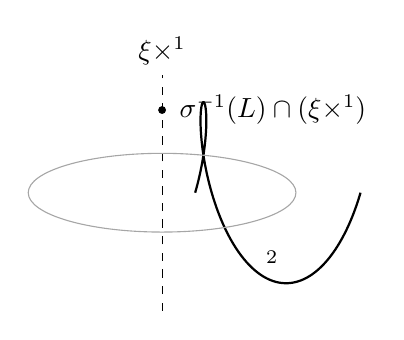
\begin{tikzpicture}[scale=1.0]
		% 螺线一圈 (示意胀开 Π → P²)
		\draw[thick, domain=0:360, samples=120, smooth, variable=\t]
			plot ({2.1*\t/360 - 1.05 + 0.42*cos(\t)}, {1.15*sin(\t)});
		% 中心轴 (ξ × P¹)
		\draw[dashed] (-1.05,-1.5) -- (-1.05,1.5) node[above] {$\xi \times \PP^1$};
		% 底部圆 (P² 的示意)
		\draw[gray!70] (-1.05,0) ellipse (1.7 and 0.5);
		\node[below] at (0.35,-0.62) {$\PP^2$};
		% 一条直线的原像与轴的交点
		\fill (-1.05,1.05) circle (0.05);
		\node[right] at (-0.95,1.05) {$\sigma^{-1}(L) \cap (\xi \times \PP^1)$};
	\end{tikzpicture}
	\caption{胀开 $\sigma: \Pi \to \PP^2$}
	\label{fig:2.4}
\end{figure}

\subsection{局部胀开}

对任意拟投影簇 $X$ 与非奇异点 $\xi \in X$, 我们现在构造一个簇 $Y$ 与映射 $\sigma: Y \to X$, 类似于 §4.1 对 $X = \PP^n$, $\xi = (1 : 0 : \cdots : 0)$ 构造的映射.

从一个辅助构造开始. 设 $X$ 是拟投影簇, $\xi \in X$ 是非奇异点, $u_1, \ldots, u_n$ 是在 $X$ 上处处正则的函数, 满足: (a) 方程 $u_1 = \cdots = u_n = 0$ 在 $X$ 中只有唯一解 $\xi$; (b) $u_1, \ldots, u_n$ 构成 $X$ 在 $\xi$ 处的局部参数组.

考虑积 $X \times \PP^{n-1}$ 及其子簇 $Y \subset X \times \PP^{n-1}$, 由满足
\[
	u_i(x)\, t_j = u_j(x)\, t_i \qquad (i, j = 1, \ldots, n)
\]
的点 $(x;\, t_1 : \cdots : t_n)$（$x \in X$, $(t_1 : \cdots : t_n) \in \PP^{n-1}$）组成. 第一投影 $X \times \PP^{n-1} \to X$ 在 $Y$ 上的限制给出的正则映射 $\sigma: Y \to X$ 称为 $X$ 的以 $\xi$ 为中心的\emph{局部胀开}.

注意这一构造一般不适用于 $X$ 是射影簇的情形, 因为它要求 $X$ 上存在非常数的处处正则函数 $u_1, \ldots, u_n$. 因此在 $X = \PP^n$ 时, 新概念并不包含前述胀开的概念. 二者的关系如下: 用 $\mathcal X \subset \PP^n$ 表示由 $x_0 \ne 0$ 定义的仿射子集, 令 $\mathcal Y = \sigma^{-1}(\mathcal X)$. 那么胀开 $\Pi \to \PP^n$ 在 $\mathcal Y$ 上诱导的映射 $\sigma: \mathcal Y \to \mathcal X$ 是一个局部胀开.

§4.1 中对 $\PP^n$ 的胀开证明的下列性质对局部胀开逐字逐句同样成立. 映射 $\sigma: Y \to X$ 正则, 且给出同构
\[
	Y \setminus (\xi \times \PP^{n-1}) \overset{\sim}{\longrightarrow} X \setminus \xi.
\]
在点 $y \in \sigma^{-1}(\xi)$ 处某个 $t_i \ne 0$, 可令 $s_j = t_j/t_i$（$j \ne i$). 此时 $Y$ 的方程取形式 $u_j = u_i s_j$（$j = 1, \ldots, n$, $j \ne i$). 由此可知 $y$ 的极大理想为
\begin{gather*}
	\mathfrak m_y = \bigl( u_1 - u_1(y), \ldots, u_n - u_n(y),\ s_1 - s_1(y), \ldots, s_n - s_n(y) \bigr) \\
	= \bigl( s_1 - s_1(y), \ldots, u_i - u_i(y), \ldots, s_n - s_n(y) \bigr),
\end{gather*}
故 $\dim \Theta_{Y,y} \le n$. 又 $\dim \overline{\sigma^{-1}(X \setminus \xi)} = n$, 故 $Y$ 在每点 $y \in \overline{\sigma^{-1}(X \setminus \xi)}$ 非奇异. 既然
\[
	Y = (\xi \times \PP^{n-1}) \cup \overline{\sigma^{-1}(X \setminus \xi)},
\]
$Y$ 或者不可约, 等于 $\sigma^{-1}(X \setminus \xi)$ 的闭包; 或者有第二个同构于 $\PP^{n-1}$ 的分支. 后一情形两个分支必相交: 否则 $\overline{\sigma^{-1}(X \setminus \xi)}$ 将在 $X \times \PP^{n-1}$ 中闭, 于是由定理~\ref{thm:projection-closed}, 其像 $X \setminus \xi \subset X$ 也闭; 而两分支的交点是奇异的, 与定理~\ref{thm:unique-component} 矛盾.

于是 $Y$ 不可约且非奇异, 且在使 $t_i \ne 0$ 的点 $y \in \sigma^{-1}(\xi)$ 处, $s_1 - s_1(y), \ldots, u_i - u_i(y), \ldots, s_n - s_n(y)$ 是局部参数.

局部胀开显然是固有映射（见定理~\ref{thm:projection-closed} 证明后的讨论）.

现在证明一个可以合理地称为``局部胀开不依赖于局部参数组 $u_1, \ldots, u_n$ 的选取''的性质.

\begin{lemma}\label{lem:blowup-independence}
	设 $v_1, \ldots, v_n$ 是 $X$ 上满足上述条件 (a) 与 (b) 的另一组函数, $\sigma': Y' \to X$ 是用 $v_1, \ldots, v_n$ 如上构造的局部胀开. 那么存在同构 $\varphi: Y \to Y'$, 使图表
	\[
		\begin{tikzcd}
			Y \ar[rr, "\varphi"] \ar[dr, swap, "\sigma"] & & Y' \ar[dl, "\sigma'"] \\
			& X &
		\end{tikzcd}
	\]
	交换.
\end{lemma}

\begin{proof}
	我们有 $Y' \subset X \times \PP^{n-1}$, 其中 $\PP^{n-1}$ 的齐次坐标记作 $t'_1, \ldots, t'_n$. 在开集 $Y \setminus \sigma^{-1}(\xi)$ 与 $Y' \setminus \sigma'^{-1}(\xi)$ 上, 令
	\begin{equation}
		\label{eq:2.28}
		\begin{split}
			\varphi(x;\, t_1 : \cdots : t_n) = (x;\, v_1(x) : \cdots : v_n(x)), \\
			\psi(x;\, t'_1 : \cdots : t'_n) = (x;\, u_1(x) : \cdots : u_n(x)).
		\end{split}
	\end{equation}
	由诸 $u_i$ 的性质 (a), $\varphi$ 与 $\psi$ 是正则映射
	\[
		\varphi: Y \setminus \sigma^{-1}(\xi) \to Y', \qquad \psi: Y' \setminus \sigma'^{-1}(\xi) \to Y.
	\]
	现在考虑 $Y$ 的使 $t_i \ne 0$ 的开集, 令 $s_j = t_j/t_i$. 既然 $v_k(\xi) = 0$ 而 $u_1, \ldots, u_n$ 是理想 $\mathfrak m_\xi$ 的一组基, 有
	\begin{equation}
		\label{eq:2.29}
		v_k = \sum_{j=1}^{n} h_{kj}\, u_j, \qquad h_{kj} \in \mathcal O_\xi.
	\end{equation}
	在我们的开集中 $u_j = u_i s_j$, 故
	\begin{equation}
		\label{eq:2.30}
		v_k = u_i \sum_{j=1}^{n} \sigma^*(h_{kj})\, s_j = u_i\, g_k, \qquad g_k = \sum_{j=1}^{n} \sigma^*(h_{kj})\, s_j.
	\end{equation}
	令 $\varphi(x;\, t_1 : \cdots : t_n) = (x;\, g_1 : \cdots : g_n)$. 显然这个映射在两处都有定义的地方与 \eqref{eq:2.28} 一致, 因为那里 $g_k = v_k/u_i$. 我们验证 $\varphi$ 正则: 必须证明 $g_1, \ldots, g_n$ 在任何点 $\eta \in \sigma^{-1}(\xi)$ 处不同时为零. 设 $g_1(\eta) = \cdots = g_n(\eta) = 0$. 既然诸 $s_j(\eta)$ 不全为零（因为 $s_i = 1$）, 由 \eqref{eq:2.30} 得 $\det|h_{kj}(\xi)| = 0$. 但 $v_k \equiv \sum h_{kj}(\xi)\, u_j \pmod{\mathfrak m_\xi^2}$, 由此将得诸 $v_k$ 在 $\mathfrak m_\xi/\mathfrak m_\xi^2$ 中线性相关, 而它们构成 $\xi$ 处的局部坐标组, 矛盾.

	于是我们定义了整体映射 $\varphi: Y \to Y'$, 类似地有映射 $\psi: Y' \to Y$. 只需在 \eqref{eq:2.28} 成立的开集上验证它们互逆, 而这是显然的. 引理证毕.
\end{proof}

\subsection{胀开下子簇的性状}

设 $X \subset \PP^N$ 是拟投影子簇, $\sigma: \Pi \to \PP^N$ 是 §4.1 定义的胀开. 我们研究子簇 $X$ 的原像 $\sigma^{-1}(X)$, 它当然是 $\Pi$ 的拟投影子簇.

\begin{theorem}\label{thm:blowup-subvariety}
	设 $X \subset \PP^N$ 是不可约拟投影簇, $X \ne \PP^N$, 且 $X$ 在 $\xi$ 处非奇异. 那么 $X$ 在以 $\xi$ 为中心的胀开下的原像 $\sigma^{-1}(X)$ 可约, 由两个分支组成:
	\begin{equation}
		\label{eq:2.31}
		\sigma^{-1}(X) = (\xi \times \PP^{N-1}) \cup Y.
	\end{equation}
	$\sigma$ 在分支 $Y$ 上的限制给出正则映射 $\sigma: Y \to X$, 它在 $x \ne \xi$ 的某邻域上是同构, 而当 $x = \xi$ 时 $\sigma^{-1}(U) \to U$ 是以 $\xi$ 为中心的局部胀开.
\end{theorem}

\begin{proof}
	用 $Y$ 表示 $\sigma^{-1}(X \setminus \xi)$ 的闭包. 既然 $\sigma^{-1}$ 在 $\PP^N \setminus \xi$ 上是同构, $\sigma^{-1}(X \setminus \xi)$ 同构于 $X \setminus \xi$, 故不可约, 于是 $Y$ 也不可约. \eqref{eq:2.31} 由定义显然: 若 $x \in X \setminus \xi$ 则 $\sigma^{-1}(x) \in Y$, 而 $\sigma^{-1}(\xi) = \xi \times \PP^{M-1}$.

	$\sigma: Y \to X$ 在 $x \ne \xi$ 的任何点的邻域上是同构这一点已经指出. 剩下研究 $\sigma: Y \to X$ 在 $\xi$ 的邻域上的情形.

	现在利用胀开可以描述为含 $\xi$ 的仿射空间 $\A^N$ 的局部胀开这一事实, 以及局部胀开对局部参数选取的独立性. 据定理~\ref{thm:subvariety-local-params}, 可选取 $\xi \in \PP^N$ 处的局部参数组 $u_1, \ldots, u_N$, 使在 $\xi$ 的某邻域中子簇 $X$ 有局部方程
	\begin{equation}
		\label{eq:2.32}
		u_{n+1} = \cdots = u_N = 0,
	\end{equation}
	且函数 $u_1, \ldots, u_n$ 构成 $X$ 在 $\xi$ 处的局部参数组. 可取 $\PP^N$ 的邻域 $U \ni \xi$ 使 $u_1, \ldots, u_N$ 满足 §4.2 引理的条件 (a) 与 (b), 于是定理的证明归结为 $X$ 由 \eqref{eq:2.32} 给出的特殊情形.

	由条件 (a), (b) 与 $u_i t_j = u_j t_i$ 得, 对 $x \ne \xi$ 有 $t_{n+1}(x) = \cdots = t_N(x) = 0$. 故 $Y$ 含于由方程
	\begin{equation}
		\label{eq:2.33}
		t_{n+1} = \cdots = t_N = 0
	\end{equation}
	与
	\begin{equation}
		\label{eq:2.34}
		u_i\, t_j = u_j\, t_i \qquad (i, j = 1, \ldots, n)
	\end{equation}
	定义的子空间 $Y' \subset X \times \PP^{M-1}$. 用 $\PP^{n-1}$ 表示 $\PP^{M-1}$ 中满足 \eqref{eq:2.33} 的点的子空间, 则 $Y' \subset X \times \PP^{n-1}$ 且在其中由 \eqref{eq:2.34} 定义. 于是 $Y'$ 正是局部胀开所得的簇. 我们已证 $Y' = \overline{\sigma^{-1}(X \setminus \xi)}$, 故 $Y = Y'$, 定理得证.
\end{proof}

现在可以给出以一点为中心的胀开的最一般定义. 设 $X \subset \PP^N$ 是拟投影簇, $\xi$ 是 $X$ 的非奇异点, $Y$ 是定理~\ref{thm:blowup-subvariety} 陈述中引入的簇, 则 $\sigma: Y \to X$ 称为 $X$ 的以 $\xi$ 为中心的胀开. 由局部胀开已证的性质可知: 若 $X$ 不可约则 $Y$ 不可约; $\sigma^{-1}(\xi) \cong \xi \times \PP^{n-1}$, 且 $\sigma^{-1}(\xi)$ 的所有点都是 $Y$ 的非奇异点.

注意当 $X$ 是曲线时胀开是同构. 于是非平凡的胀开是高维代数几何的典型现象.

\subsection{例外子簇}

胀开的例子显示了代数曲线与维数 $n > 1$ 的簇之间原则性的差别: 非奇异射影曲线之间的双有理映射是同构, 而胀开表明在高维情形并非如此.

注意胀开的一个特点: 它是正则映射, 之所以不是同构, 只是因为有理映射 $\sigma^{-1}$ 在点 $\xi$ 处不正则.

本节研究映射 $f: X \to Y$, 其中 $f$ 是正则的双有理映射, 即 $g = f^{-1}: Y \to X$ 是有理而非正则的映射. 在胀开的例子中我们看到, $Y$ 中的余维 $1$ 子簇被收缩为点 $\xi$. 我们证明在这一情形总有同样的性质成立.

\begin{theorem}\label{thm:exceptional}
	设 $f: X \to Y$ 是正则的双有理映射. 对 $x \in X$, 设 $y = f(x)$ 是 $Y$ 的非奇异点而逆映射 $g = f^{-1}$ 在 $y$ 处不正则. 那么存在子簇 $Z \subset X$, $Z \ni x$, 使 $\operatorname{codim} Z = 1$ 而 $\operatorname{codim} f(Z) \ge 2$.
\end{theorem}

\begin{proof}
	必要时把 $X$ 换成 $x$ 的仿射邻域, 可设 $X$ 仿射. 设 $X \subset \A^N$, 坐标为 $t_1, \ldots, t_N$, 而 $g = f^{-1}$ 是由 $t_i = g_i$（$i = 1, \ldots, N$, $g_i \in k(Y)$）给出的映射. 显然 $g_i = g^*(t_i)$; 既然 $g$ 在 $y$ 处不正则, 至少某个函数 $g_i$ 在 $y$ 处不正则. 设其为 $g_1$, 于是 $g_1 \notin \mathcal O_y$.

	把 $g_1$ 写成 $g_1 = u/v$（$u, v \in \mathcal O_y$, $v(y) = 0$）; 既然 $\mathcal O_y$ 是唯一分解整环（因为 $y$ 非奇异）, 可设 $u$ 与 $v$ 没有公因子. 由 $g = f^{-1}$ 得 $t_1 = f^*(g_1) = f^*(u)/f^*(v)$, 故
	\begin{equation}
		\label{eq:2.35}
		f^*(v)\, t_1 = f^*(u).
	\end{equation}
	现在 $f^*(v)(x) = v(y) = 0$, 故 $x \in V(f^*(v))$. 令 $Z = V(f^*(v))$. 由相交维数定理 $\operatorname{codim} Z = 1$, 且 $Z \ni x$ 故非空. 由 \eqref{eq:2.35} 得 $f^*(u)$ 在 $Z$ 上为零, 于是 $u$ 在 $f(Z)$ 上为零, 故 $f(Z) \subset V(u) \cap V(v)$.

	剩下验证 $\operatorname{codim}(V(u) \cap V(v)) \ge 2$. 若 $V(u) \cap V(v)$ 含有满足 $y \in Y'$ 且 $\operatorname{codim} Y' = 1$ 的分支 $Y'$, 则由定理~\ref{thm:codim1-local-eq}, $Y'$ 有局部方程 $h$, 这意味着 $u, v \in (h)$, 与 $u, v$ 在 $\mathcal O_y$ 中无公因子的假设矛盾. 定理证毕.
\end{proof}

\begin{definition}[例外子簇]\label{def:exceptional}
	设 $f: X \to Y$ 是正则的双有理映射. 子簇 $Z \subset X$ 称为 $f$ 的\emph{例外子簇}\index{liwai zicu@例外子簇}, 如果 $\operatorname{codim} Z = 1$ 而 $\operatorname{codim} f(Z) \ge 2$.
\end{definition}

\begin{corollary}\label{cor:exceptional-exists}
	非奇异簇之间非同构的正则双有理映射 $f: X \to Y$ 必有例外子簇.
\end{corollary}

\begin{corollary}\label{cor:curve-open-iso}
	设 $f: X \to Y$ 是曲线 $X$ 与 $Y$ 之间的正则双有理映射, 且 $Y$ 非奇异; 那么 $f(X)$ 在 $Y$ 中开, 且 $f$ 给出 $X$ 到 $f(X)$ 的同构.
\end{corollary}

\begin{proof}
	由 $X$ 与 $Y$ 有同构的开子集 $U$ 与 $V$（第一章命题~\ref{prop:birational-opens}）可得 $f(X)$ 在 $Y$ 中开: 事实上, 既然 $f(U) = V$ 是去掉有限多个点得到的, $f(X)$ 更加如此, 故在 $Y$ 中开. 若 $f: X \to f(X)$ 不是同构, 则与定理~\ref{thm:exceptional} 矛盾, 因为在我们的情形只有空集的余维数 $\ge 2$. 推论证毕.
\end{proof}

\subsection{同构与双有理等价}

考虑拟投影簇的双有理等价类, 即彼此双有理等价的全部拟投影簇组成的类. 该类的一个代表称为\emph{模型}.

在下面 §5.3 中我们将证明: 每个代数曲线的双有理等价类中存在非奇异射影模型 $X_0$. 定理~\ref{thm:rational-map-codim2} 与推论~\ref{cor:curves-birational-iso} 断言每个双有理等价类中这样的模型在同构意义下至多一个. 于是, 把曲线的双有理等价类对应到其中唯一的非奇异射影模型, 就把曲线按双有理等价的分类问题化为非奇异射影曲线按同构的分类问题.

代数曲线 $X$ 的函数域 $k(X)$ 是 $k$ 上由有限多个元素生成且超越次数为 $1$ 的扩域. 于是我们可以在这样的域 $K$ 与非奇异射影曲线 $X$ 之间建立一一对应, 对应由 $K = k(X)$ 给出; 也称 $X$ 是 $K$ 的一个模型.

可以尝试直接从域 $K$ 的代数性质找出非奇异射影模型 $X$. 把问题提得更确切: 点 $x \in X$ 的局部环 $\mathcal O_x$ 在 $K$ 中如何刻画? 容易看出, 每个点 $x \in X$ 的局部环 $\mathcal O_x$ 都有下列性质:
\begin{compactenum}[(1)]
	\item $\mathcal O$ 是 $K$ 的子环且 $k \subsetneq \mathcal O \subsetneq K$;
	\item $\mathcal O$ 是局部环, 且其极大理想 $\mathfrak m$ 是主理想, 即 $\mathfrak m = (u)$;
	\item $K$ 等于 $\mathcal O$ 的分式域.
\end{compactenum}
可以证明（见习题 7--9）: 满足 (1)--(3) 的任何子环 $\mathcal O \subset K$ 都是某点 $x \in X$ 的局部环 $\mathcal O_x$. 于是非奇异射影模型 $X$ 是万有的: 它穷尽了 $K$ 中满足自然条件 (1)--(3) 的全部局部环.

这些问题在维数 $n > 1$ 时如何? 就非奇异射影模型的存在性而言, 情况相当好: $n = 2$ 或 $3$ 时已经证明（Walker 与 Zariski 在特征 $0$, Abhyankar 在特征 $p > 5$）, 任意 $n$ 在特征 $0$ 时也已证明（Hironaka）. 对任意域与任意 $n$, 非奇异射影模型的存在性看来极有可能成立. 相反, 非奇异射影模型的唯一性却是 $n = 1$ 情形独有的特性; 这从射影平面 $\PP^2$ 与非奇异二次曲面 $Q \subset \PP^3$ 的例子已经可以看出: 它们双有理等价而不同构.

有人可能问: 是否在每个双有理等价类中存在一个万有模型 $X$, 使其点 $x \in X$ 的局部环 $\mathcal O_x$ 穷尽域 $K = k(X)$ 中满足 (1), (2), (3) 的全部局部子环, 其中 $n = 1$ 情形条件 (2) 中的 $\mathfrak m = (u)$ 换成 $n$ 维版本 $\mathfrak m = (u_1, \ldots, u_n)$? 然而由于同样的理由, 这样的模型不可能存在. 事实上, 若 $\sigma: X' \to X$ 是 $X$ 的以 $\xi$ 为中心的胀开, 则点 $y \in \sigma^{-1}(\xi)$ 的局部环不等于任何点 $x \in X$ 的局部环 $\mathcal O_x$; 读者容易把这作为练习证明. 当然, 把一个双有理等价类的全部模型的全部非奇异点并在一起确实得到一个具有上述万有性的对象, 即所谓 Zariski Riemann 面, 但这个对象不是有限维代数簇. 关于这个``无穷维模型''的某些信息见 Zariski--Samuel \cite[第 VI 章第 17 节]{zariski-samuel1960}.

既然不存在特别的模型, 就产生了研究每个双有理等价类中各非奇异射影模型之间关系的问题. 我们在此不加证明地叙述这一领域迄今已知的主要结果. 以下所考虑的簇都设为不可约, 非奇异且射影的.

从两个定义开始. 称模型 $X'$ 支配 $X$, 如果存在正则双有理映射 $f: X' \to X$. 簇 $X$ 称为\emph{相对极小模型}\index{xiangdui jixiao moxing@相对极小模型}, 如果它不支配任何与它自身不同构的簇. 例如, 非奇异射影曲线总是相对极小模型. 由定理~\ref{thm:exceptional}, 簇是相对极小模型当且仅当它不含任何例外子簇.

可以证明每个簇至少支配一个相对极小模型, 于是每个双有理等价类至少含一个相对极小模型. 随之产生相对极小模型的唯一性问题: 若每个双有理等价类都有唯一的相对极小模型, 就又把簇的双有理分类化为按同构的分类. 然而对 $n > 1$ 这行不通. 例子由射影平面 $\PP^2$ 与非奇异二次曲面 $Q \subset \PP^3$ 提供: 如我们所知它们双有理等价, 即属于同一双有理等价类; 我们证明 $\PP^2$ 与 $Q$ 都是相对极小模型, 即都不含例外曲线. 既然 $\PP^2$ 与 $Q$ 不同构（比较推论~\ref{cor:curves-meet} 后的讨论）, 这就给出所需的例子.

在我们的情形, 不可约例外曲线 $C \subset X$ 应被正则双有理映射 $f: X \to Y$ 收缩为一点, 即 $f(C) = y \in Y$; 这里 $X$ 与 $Y$ 是射影曲面. 这种曲线具有一系列非常特殊的性质（``例外''之名即由此而来）, 我们只讨论其中之一.

由定理~\ref{thm:rational-map-codim2}, 映射 $f^{-1}$ 只在有限多个点 $y_i \in Y$ 处不正则. 设 $U$ 是 $y$ 的足够小的仿射邻域, 使 $f^{-1}$ 在 $U$ 中除 $y$ 外的每点都正则. 令 $V = f^{-1}(U)$, $C = f^{-1}(y)$. 显然 $V$ 是 $X$ 的开子集且 $V \supset C$. 我们证明 $V$ 不含任何在 $X$ 中闭且不含于 $C$ 的不可约曲线 $C'$. 事实上, $C'$ 是射影曲线, 其像 $f(C')$ 也是射影的; 但 $f(C') \subset U$ 是仿射的. 由定理~\ref{thm:projection-closed} 与推论~\ref{cor:projective-to-affine}, 这只在 $f(C') = y'$ 为一点时才可能. 若 $y' \ne y$, 则因 $f^{-1}$ 是同构, $C'$ 也应是一点; 若 $y' = y$, 则 $C' \subset f^{-1}(y) = C$.

于是 $C$ 在 $X$ 中是孤立的, 意即存在 $C$ 的邻域 $V$, 除含于 $C$ 的曲线外不含任何不可约射影曲线. 换言之, 不可能``把 $C$ 稍微挪动一下''. 由此可推出许多曲面不含例外曲线.

例如, 设 $X = \PP^2$ 而 $C$ 是例外曲线, $C \subset V = \PP^2 \setminus D$. 那么 $\dim D = 0$; 因为否则由相交维数定理, $C$ 与 $D$ 将相交. 但若 $\dim D = 0$, 即 $D$ 是有限点集, 则 $V$ 含有任意多条与 $D$ 不相交的曲线 $C$, 例如直线.

再设 $X = Q$ 是 $\PP^3$ 中的非奇异二次曲面. 这里利用把 $Q$ 变为自身的射影变换群 $G$ 的存在性. 回忆 $G$ 的变换由满足关系 ${}^t A F A = F$ 的 $4 \times 4$ 矩阵给出, 其中 $F$ 是定义 $Q$ 的二次型的矩阵. 由此可知 $G$ 是全部 $4 \times 4$ 矩阵空间中的代数簇, 以下就把 $G$ 视为仿射代数簇. 容易看出 $G$ 传递地作用于 $Q$.

若 $C$ 是曲线且 $C \subset Q \setminus D$, 则构造变换 $\varphi \in G$ 使 $\varphi(C) \not\subset C$ 且 $\varphi(C) \subset Q \setminus D$, 与上面得到的例外曲线的性质矛盾. 为此只需证明使 $\varphi(C) \cap D \ne \emptyset$ 的 $\varphi \in G$ 的集合是闭的; 于是在恒等变换 $e \in G$ 的整个邻域中的元素都具有所需性质. 为描述使 $\varphi(C) \cap D \ne \emptyset$ 的元素 $\varphi \in G$ 的集合 $S$, 考虑直积 $G \times Q$ 及其中由满足 $x \in C$ 且 $\varphi(x) \in D$ 的对 $(\varphi, x)$ 组成的子集 $\Gamma$; 显然 $\Gamma$ 闭. 若 $f: G \times Q \to G$ 是投影, 则 $S = f(\Gamma)$, 而由定理~\ref{thm:image-closed}, $f(\Gamma)$ 闭. 这就完成了 $Q$ 是相对极小模型从而存在两个不同相对极小模型的证明.

因此更加令人惊讶的是: 对代数曲面, 只要排除一些特殊类型的曲面, 极小模型的唯一性确实成立. 即如 Enriques 所证: 只要双有理等价类不含形如 $C \times \PP^1$（$C$ 为代数曲线）的曲面, 曲面的双有理等价类就含唯一的相对极小模型.（与 $C \times \PP^1$ 双有理等价的曲面称为直纹面.）Enriques 定理的证明见 Shafarevich \cite[第 II 章]{shafarevich1994} 或 Barth--Peters--van de Ven \cite{barth1984}.

近来在维数 $\ge 3$ 的极小模型理论的构造方向上有重大进展. 在这种情形, 极小模型不能在非奇异簇的类中存在, 但有理由期望: 若允许一类相当受控的奇点, 理论可以推广. 为此见综述 Kawamata--Matsuda--Matsuki \cite{kmm1987} 与 Shokurov \cite{shokurov1985}.

\subsection{第 4 节习题}

\begin{compactenum}
	\item 设 $\dim X = 2$, $\xi \in X$ 是非奇异点. 设 $C_1, C_2 \subset X$ 是经过 $\xi$ 且在该处非奇异的两条曲线, $\sigma: Y \to X$ 是以 $\xi$ 为中心的胀开, 令 $C'_i = \overline{\sigma^{-1}(C_i \setminus \xi)}$, $Z = \sigma^{-1}(\xi)$. 证明 $C'_1 \cap Z = C'_2 \cap Z$ 当且仅当 $C_1$ 与 $C_2$ 在 $\xi$ 处相切.
	\item 设 $\dim X = 2$, $\xi \in X$ 是非奇异点. 设 $C$ 是经过 $\xi$ 的曲线, $f$ 是 $C$ 在 $\xi$ 的某邻域中的局部方程. 在 $\xi$ 处的局部参数 $u, v$ 下, 设 $f \equiv \prod_{i=1}^{r} (\alpha_i u + \beta_i v)^{l_i} \pmod{\mathfrak m_\xi^{k+1}}$, 其中 $k = \sum l_i$ 且诸型 $\alpha_i u + \beta_i v$ 两两不成比例. 如习题 1 设 $\sigma: Y \to X$, $C' = \overline{\sigma^{-1}(C \setminus \xi)}$. 证明 $C' \cap Z$ 由 $r$ 个点组成.
	\item 沿用习题 2 的记号, 并设 $f \equiv (\alpha_1 u + \beta_1 v)(\alpha_2 u + \beta_2 v) \pmod{\mathfrak m_\xi^3}$, 其中两个线性型不成比例. 证明 $C' \cap Z$ 的两个点都是 $C'$ 的非奇异点.
	\item 考虑由
	\[
		\varphi(x_0 : x_1 : x_2) = (x_0 x_1 : x_0 x_2 : x_1^2 : x_1 x_2 : x_2^2)
	\]
	给出的有理映射 $\varphi: \PP^2 \to \PP^4$. 证明 $\varphi$ 是到曲面 $\varphi(\PP^2)$ 的双有理映射, 且逆映射 $\varphi(\PP^2) \to \PP^2$ 与胀开一致.
	\item 仿照习题 4, 研究由除 $x_0^3, x_1^3, x_2^3$ 以外的全部三次单项式定义的映射 $\varphi: \PP^2 \to \PP^6$.
	\item 对任何 $n \ge 2$, 构造 $n$ 维非奇异簇之间的正则双有理映射 $f: X \to Y$ 的例子, 使之具有例外余维 $1$ 子簇 $Z$, 其像 $f(Z) \subset Y$ 的余维数为 $2$.
	\item 设 $X$ 是非奇异射影曲线, $\mathcal O \subset k(X)$ 是函数域 $k(X)$ 中满足 §4.5 条件 (1)--(3) 的局部子环. 证明: 对任何 $u \in k(X)$, 或者 $u \in \mathcal O$, 或者 $u^{-1} \in \mathcal O$. 设 $X \subset \PP^n$, $x_0, \ldots, x_n$ 是 $\PP^n$ 的齐次坐标. 证明存在 $i$ 使对 $j = 0, \ldots, n$ 有 $x_j/x_i \in \mathcal O$.
	\item 沿用习题 7 的记号. 设 $X'$ 是仿射曲线 $X' = X \cap \A^n_i$. 证明 $k[X'] \subset \mathcal O$, 且 $\mathcal O$ 的极大理想 $\mathfrak m$ 满足: $k[X] \cap \mathfrak m$ 是某点 $x \in X'$ 的理想, 且 $\mathcal O_x \subset \mathcal O$.
	\item 证明: 若 $\mathcal O_1$ 与 $\mathcal O_2$ 是满足 §4.5 条件 (1)--(3) 的两个子环且 $\mathcal O_1 \subset \mathcal O_2$, 则 $\mathcal O_1 = \mathcal O_2$. 由此并利用习题 7--8 的结果证明 $\mathcal O = \mathcal O_x$（沿用习题 8 的记号）.
	\item 设 $V \subset \A^3$ 是由 $xy = z^2$ 定义的二次锥面; 设 $X' \to \A^3$ 是以原点为中心的 $\A^3$ 的胀开, $V'$ 是 $\sigma^{-1}(V \setminus 0)$ 在 $X'$ 中的闭包. 证明 $V'$ 非奇异, 且原点在 $\sigma: V' \to V$ 下的原像是一条非奇异有理曲线.
\end{compactenum}
